%% Copernicus Publications Manuscript Preparation Template for LaTeX Submissions
%% ---------------------------------
%% This template should be used for copernicus.cls
%% The class file and some style files are bundled in the Copernicus Latex Package, which can be downloaded from the different journal webpages.
%% For further assistance please contact Copernicus Publications at: production@copernicus.org
%% https://publications.copernicus.org/for_authors/manuscript_preparation.html


%% Please use the following documentclass and journal abbreviations for preprints and final revised papers.

%% 2-column papers and preprints
\documentclass[amt, manuscript]{copernicus}

\newcommand{\todo}[1]{{\color{red} #1}}

%% \usepackage commands included in the copernicus.cls:
%\usepackage[german, english]{babel}
\usepackage{tabularx}
%\usepackage{cancel}
%\usepackage{multirow}
%\usepackage{supertabular}
%\usepackage{algorithmic}
%\usepackage{algorithm}
\usepackage{amsthm}
\usepackage{float}
%\usepackage{subfig}
%\usepackage{rotating}


\begin{document}

\title{Implications of ice hydrometeor orientation on IWP retrievals using GMI polarimetric measurements}


% \Author[affil]{given_name}{surname}

\Author[1]{Inderpreet}{Kaur}
\Author[1]{Patrick}{Eriksson}
\Author[1]{Vasileios}{Barlakas}
\Author[1]{Simon}{Pfreundschuh}


\affil[1]{Chalmers University of Technology, Gothenburg, Sweden}

%% The [] brackets identify the author with the corresponding affiliation. 1, 2, 3, etc. should be inserted.

%% If an author is deceased, please mark the respective author name(s) with a dagger, e.g. "\Author[2,$\dag$]{Anton}{Smith}", and add a further "\affil[$\dag$]{deceased, 1 July 2019}".

%% If authors contributed equally, please mark the respective author names with an asterisk, e.g. "\Author[2,*]{Anton}{Smith}" and "\Author[3,*]{Bradley}{Miller}" and add a further affiliation: "\affil[*]{These authors contributed equally to this work.}".


\correspondence{Inderpreet Kaur (kauri@chalmers.se)}

\runningtitle{Ice water path retrievals}

\runningauthor{Kaur}





\received{}
\pubdiscuss{} %% only important for two-stage journals
\revised{}
\accepted{}
\published{}

%% These dates will be inserted by Copernicus Publications during the typesetting process.


\firstpage{1}

\maketitle



\begin{abstract}
Existing datasets of ice water path (IWP) based on passive observations 
either show a clear low bias compared to radar retrievals or are 
completely empirical. It is here shown that much more accurate 
physically-based passive retrievals are possible. The high-frequency 
channels of the GMI radiometer are used for demonstration. The progress 
is mainly achieved by detailed radiative transfer simulations, that 
closely mimic the real observations statistically. A novel aspect is 
that particle orientation is considered and polarisation signatures in 
the observations can be exploited. The simulations are used as input to 
a machine learning retrieval algorithm. Both the simulations and the 
inversions are made in a Bayesian fashion. As a consequence, reasonably 
complete distributions of IWP are provided and the retrievals can be 
considered as all-sky in contrast to most other datasets, limited to 
either the low or high end of the IWP distribution. Example results and 
applications are shown. For example, a clear diurnal variation of IWP in 
the Tropics is confirmed. So far satellite-based cloud radars are only 
nadir-pointing while these passive retrievals have a swath width of ? 
km, and this broad coverage should provide opportunities to assess model 
cloud parametrisations in new manners

\end{abstract}


\copyrightstatement{TEXT} %% This section is optional and can be used for copyright transfers.


\introduction  %% \introduction

Ice clouds have a profound impact the Earth's radiation balance. They reflect the short and long wave radiation and emit long wave radiation contributing to the Earth’s energy balance and hydrological cycle \citep{liou:influ:86}. The total radiative forcing is dependent both on the microphysical and macrophysical properties, such as, the spatial distribution of ice particles, particle orientation, ice water content, etc. However, due to the complex vertical and spatio-temporal heterogeneity associated with ice clouds, the knowledge on the global distribution of atmospheric ice is deficient and not well captured by the models \citep{wilson:theim:00}. Significant uncertainties, in both meteorological and climate models, are inflicted by the simplifications introduced to resolve the complex structures \citep{reinhardt:impac:04}.


Ice water content (IWC)  is a key variable used to measure the atmospheric ice. It is defined as the bulk mass of ice in the atmosphere and the column integrated bulk mass is the ice water path (IWP). The existing space based retrieval systems measuring IWC/IWP, use observations from either active or passive microwave sensors or exploit the synergies between the two. The synergy between the 94\,\,GHz radar onboard Cloudsat and CALIPSO lidar provides the most accurate global distribution of atmospheric ice, especially for the tropical ice clouds \citep{protat:theev:10}. This combination can sense ice hydrometeors ranging from thin cirrus to precipitating ice \citep{stephens:cloud:18}. However, the limited spatio-temporal sampling cannot fully resolve the  variability of atmospheric ice on both local and global scales. 

Among passive microwave measurements, the millimeter (mm) wavelengths have been proven to be suitable for measuring cloud parameters. With wider swath and ability to see through the cloud microwaves observations can capture the mesoscale systems. For example, \citet{gong:cloud:14} describe an empirical model to retrieve IWP from Microwave Humidty Sounder (MHS) high frequency channels. The Synergistic Passive Atmospheric Retrieval Experiment-ICE (Spare-Ice) product \citet{holl:spare:14} is another empirical attempt which combines optical,microwave and infrared sensors to retrieve IWP. The usage infrared sensors can account for smaller ice particles in the cloud but they cannot sense the entire water column. 

The global atmopsheric ice estimates from passive microwave sensors have proven to be successful capturing the diurnal cycle and interseasonal fluctuations. However, there exists inconsistency between different cloud ice observations, thus leading to model uncertainties. A detailed comparison of different space borne IWP measurements by \citet{duncan:anupd:18, eliasson:asses:11} highlights that large discrepancies exist between different IWP estimates as the space-borne remote sensing techniques still cannot fully resolve the atmospheric ice properties. The limitations associated with sensor sensitivities and the oversimplified microphysical assumptions are mostly to blame. The sensor limitations will be overcome to a certain extent with the launch of new sensors like Ice Cloud Imager (ICI) measuring and sub-millimeter (sub-mm) wavelengths. ICI shall bridge the sensitivity gap between microwave and infrared sensors. Studies ....


However another aspect, though recognised in literature, but mostly neglected in IWP retrieval algorithms is the benefits of using dual-polarisation measurements. Most IWP retrieval studies are either based on instruments lacking dual-polarisation, or include only one of the dual polarisation channels. Thus focussing only on the radiometric intensity of the signals. The ice hydrometeors exhibit dichroism effects resulting in polarization difference (PD) between the radiances measured by horizontal(H) and vertical(V) polarizations. The PD exhibited by oriented particles is generally higher than the randomly oriented ones. Constraining the microphysical assumptions to one or few habits and neglecting  orientation effects contributes to a non-zero bias in the retrievals. High inaccuracies also are connected to areas with large PD. For example, \citet{gong:micro:17} and \citep{miao:thepo:03} argue that retrieval of cloud ice has a strong connection to the polarimetric difference introduced by oriented particles, particularly for regions with convective outflow. 

The physically based retrieval techniques associate the simulated brightness temperatures to the ice cloud structures, but most radiative transfer based retrieval algorithms, focusing on ice clouds, assume spherical or randomly oriented hydrometeors, e.g. \citep{evans:icecl:05, Zhao:retri:02}. The simplifications are often introduced to reduce computational loads, but at the same time, properties of ice-hydrometeors are still not fully understood.

%  When particles in ice clouds change from horizontally to randomly oriented, the brightness temperature changes up to 6 K. An accurate IWPretrieval therefore would require dual-polarized measurements for particle orientation information.

Zeroing on an ice model incorporating accurate ice model remains a challenge, however, microwave sensors measuring different polarizations can help in inferring the properties of ice hydrometeors. The space borne sensors can provide accurate measures of the polarimetric differences and their potential in retrieval of ice cloud properties have have been long recognised. For example, \citep{coy:sensi:20}, have shown  that incorporating polarimetric measurements improve the retrievals of ice cloud microphysics such as particle effective diameter (D$_{eff}$), while \citep{hioki:degre:16} analyse the ice particle surface roughness from polarimetric observations. However, there is a general lack of  IWC and IWP retrieval methods taking PD into account.

In this study, we explore the benefits of incorporating polarimetric measurements for retrievals of IWP using Global Precipitation Measurement (GPM) Microwave Imager (GMI). We aim for physical based measurements of IWP from passive microwave instruments, which can be bias-free and better performing than existing reanalyses and satellite based products. Currently, GMI is the only sensor which senses in dual polarisation mode above 100\,\,GHz. The Bayesian retrieval algorithm utilized by GPM for precipiation is also used for compute IWP from precipitating hydrometeors. The ice hydrometeors are not covered as the apriori database is generated for hydrometeor profiles covered by GPM Dual Precipitraion radar (DPR), which is sensitive only to precipitating hydrometeors. 

We apply a Bayesian machine learning algorithm, Quantile Regression Neural Network (QRNN) \citep{pfreundschuh:aneur:18} to retrieve IWP from a database of atmospheric profiles generated using radiative transfer model. As a first step, a database representing the GMI measurements for a variety of atmospheric conditions is created. We avoid the ice-scattering calculations but the impact of polarisation is introduced using the scheme proposed by \citet{barlakas:intro:21}. They had introduced a simple scaling factor to mimic the effects of hydrometeor orientation. In this study, the simple scaling factor is extended to cover different magnitudes of polarimetric signatures observed by the Global Precipitation Measurement (GPM) Microwave Imager (GMI) 166 GHz channels. Further, the retrieval is applied to real GMI measurements. We investigate the sensitivity of retrieved IWP to polarization differences and  quantify the errors arsing due to assumption of unpolarised signals. 

\section{Satellite and model data}

\subsection{GPM GMI}
The GPM GMI instrument is a conical microwave radiometer, which provides a near global coverage of the precipitation estimates. It has a swath of 885\,\,km  and an earth incidence angle of 52.8$^{\circ}$. It instrument has thirteen microwave channels ranging from 10\,\,GHz to 183\,\,GHz which are sensitive to the different forms of precipitation. In this study, we use only the four high frequency measurements between 166 GHz and 183 GHz (Table~\ref{tab:gmi_channels}). These channels are sensitive to the precipitating ice and water vapour.

The GMI datasets used in this study are Level-1 (L1B) TBs. The details of L1B algorithm are found in \citet{}. L1B radiances are geolocated and calibrated Level 0 counts at native resolution. 




%\subsection{Cloudsat}
%CloudSat is a sun-synchronous satellite which is part of the A-train constellation and has been providing information on the vertical structure of clouds and aerosols, since 2006. It carries a 96\,\,GHz Cloud Profiling Radar (CPR) to measure the backscattering by clouds. It has a vertical resolution of 485\,\,km, and 1.8\,\,km along-track and 1.2\,\,km cross-track resolution. 

%\subsection{ERA5}

%ERA5 is global reanalysis data provided by European Centre for Medium-Range Weather Forecasts (ECMWF). The reanalysis combines model data with observations to provide hourly estimates of a large number of atmospheric, ocean and land-surface variables . In this study, we use multiple ERA5 atmospheric and surface parameters for generation of atmospheric scenes to be used as inputs to radiative transfer simulations described in sect.~\ref{sec:atm_scenes}. The parameters used here are temperature, cloud liquid water content, specific humidity, 2\,\,m temperature, 10\,\,m U wind, 10\,\,V wind, land sea mask, snow depth, sea ice cover, surface elevation. 


\subsection{Atmospheric scenarios}
\label{sec:atm_scenes}

A bulk database of two-dimensional atmospheric scenes is created based on Cloudsat radar reflectivities \citep{marchand:hydro:08} and ERA5 atmospheric and surface parameters \citep{era5:18}. The radar reflectivities are inverted to obtain vertical profiles of ice hydrometeors and rain, by assuming a particle model(described in sect.~\ref{sec:arts_setup}), while the ERA5 data (e.g. temperature, cloud liquid water content, 10\,\,m wind, specific humidity, 2\,\,m temperature, \dots) provide the background data.

ERA5 data are collocated in space and time with the ascending and descending orbits of Cloudsat. The latitudinal grid is derived from Cloudsat orbit, while a custom vertical grid from -700\,\,m to 20000\,\,m is defined. The vertical grid spacing is 125\,\,m upto 8\,\,km and 250\,\, beyond 8\,\,km. Land and water are classified using ERA5 land sea mask. Furthermore, the locations with snow depth larger than 0.002\,\,m are classified as snow. The seaice cover is used to classify the seaice surface type. For brevity, we assume that seaice locations are covered with snow, thus the same snow-emisivity model (Sect.~\ref{sec:snow_emissivity}) is valid. For each Cloudsat orbit,  a random selection of seaice is made to The randomness helps to avoid an over-representation of the snow covered seaice. 

All values liquid water content below $10^{-8}$ or at temperature lower than 248\,\,K are also set to zero. Variation in Oxygen and Nitrogen with the amount of water vapour in the air is also considered.  

In 2011, CPR suffered from a battery anomaly and has operated in daylight-only mode since then. In order to avoid any bias due to limited temporal coverage, we select random CloudSat profiles from 2009. The data is constrained between $65^{\circ}$S and $65^{\circ}$N to match the GMI latitudinal coverage. 


\section{Tools and Methodology}

\subsection{Radiative Transfer Simulations}
\label{sec:rt_simulations}

\subsubsection{ARTS setup}
\label{sec:arts_setup}
All forward simulations are performed with Atmospheric Radiative Transfer System \citep{eriksson:arts2:11}. The two-dimensional atmosphere is approximated using an independent beam approximation as utilized in works by \citet{ekelund2020using, eriksson:towar:20}. 
The radar reflectivities are converted to bulk properties: IWC and rain water content (RWC), using a dbZ-based model system as described by \citet{ekelund2020using}. The microphysical assumptions are described below in Sect.~\ref{sec:hydrometeor_prop}. The temperature field is used to make the differentiation between liquid and ice hydrometeors. All hydrometeors below 0$^{\circ}$ are classified as ice and vice-versa. The radar measurements are inverted using an onion peeling concept. The method  divides the atmosphere into layers and for each layer the measurements are inverted using an IWC-dbZ table. The attenuation effects from hydrometeors and absorbing specied are also considered. To avoid spurious water contents due to surface clutter, a clutter zone at 1.2\,\,km land and 0.6\,\,km over water is defined. All retrievals below this zone are rejected and instead the value just above the clutter zone is used as a fill value. 

%Additionally, all retrievals above \todo{...} are assumed to be erroneous and rejected.   

The land and water/ocean emissivities are taken from Tool to Estimate Land-Surface Emissivities at Microwave frequencies (TELSEM; \citep{aires2011tool} and  Tool to Estimate Sea-Surface Emissivity from Microwaves to sub-Millimeter waves (TESSEM;
\citep{prigent2017sea}, respectively. The snow and seaice emissivities are calculated using an empirical emissivity model described in Sect.~\ref{sec:snow_emissivity}.

All simulations are performed in ``all-sky'' mode with 53$^{\circ}$ incidence angle. Only high frequency GMI channels, ie. 166V, 166H, 183$\pm$3, 183$\pm$7 are simulated. The GMI antenna pattern is assumed to be a Gaussian footprint with full width at half maximum of 7\,\,km. Multiple pencil beam simulations are averaged over this pattern to yield the antenna brightness temperatures.   

\subsubsection{Hydrometeor properties}
\label{sec:hydrometeor_prop}

Three types of hydrometeors are considered for the radiative transfer calculation: cloud ice, rain and liquid clouds. The inversion of Cloudsat reflectivities to IWC, is largely dependent on the assumed microphysical properties, thus two different ice habits are applied: large plate aggregate and evans snow aggregate. 

Both particle habits are applied separately to generate two databases.
The single scattering data are taken from ARTS single scattering database provided by \citet{eriksson:agene:18} and the particle size distribution (PSD) developed by \citet{field:snows:07} is used. F07 has two different distributions for tropics and midlatitudes, but here we have used the tropical setting, further denoted as F07T. 

Rain is assumed as a liquid sphere and the PSD is calculated using Marshall Palmer size distribution \citep{marshall:thedi:48}. The liquid clouds is assumed to be totally absorbing and their scattering effects neglected. For liquid clouds the absorption model by \citet{ellison2007permittivity} is followed.  


\subsubsection{Polarisation correction}
\label{sec:scaling_factor}

In this study, both azimuthally random orientation (ARO)  and total random orientation (TRO) hydrometeors are simulated. The existing scattering database of azimuthally randomly oriented (ARO) particles \citep{brath:micro:20} is not comprehensive. It contains two habits, but as one habit is only valid for relatively small particles (the plate habit) and the second (the aggregate habit) does not cover small particles. In practice, these two habits have to combined to effectively simulate a single habit. Additionally, simulating ARO particles inside radiative transfer is computationally expensive.

Nevertheless, there is an alternate way to approximate the hydrometeor orientation. In \citet{barlakas:intro:21} it is shown that the impact of particle orientation can be approximated by scattering data calculated for totally random orientation (TRO). The scheme was tested with RTTOV-SCATT and is available as an option in the latest RTTOV version. The polarisation effects observed by conically scanning instruments, introduced by oriented particles \citep{gong:micro:17} \citep{prigent} , are mimicked by a simple scaling factor. For TRO particles, there is no difference in the extinction between the two polarisations. However, oriented hydrometeors introduce differences between the two, and the correction factor is a simple way to approximate this effect. To model the effect of ARO particles, a correction factor ($\alpha$) is used to increase and decrease the layer optical thickness ($\tau$) in the horizontal (H) and vertical (V) 
polarised channels, respectively, and the ratio of the modified layer optical thickness gives the polarisation ratio:

\begin{eqnarray}
\rho = \frac{\tau_H}{\tau_V} = \frac{1+\alpha}{1-\alpha}
\end{eqnarray}

The factor $\alpha$ $(>= 0)$  weakens the extinction at V-polarisation and strengthens it for H-polarisation. For TRO particles, $\alpha$ is equal to one, and for ARO, within the frameworks of RTTOV-SCATT, the best estimate is suggested as 1.4 ($\alpha$=1.67, for 166\,\,GHz, \citep{barlakas:intro:21}).

In this study, we extend this scheme within the ARTS setup for high-frequency channels of GMI, but with slight modifications. The polarisation ratios discussed in \citep{barlakas:intro:21}) cannot be used directly in our study. They calculated the optimal value of $\rho$ on ``superobbed'' observations. That is, the GMI observations were averaged to a coarser scale to meet the model resolution. However, on a footprint resolution, the effective value of $\rho$ can be different.  Intuitively, the value should still be close to as suggested in the study, but requires comparison of the distributions of the forward modelled radiances and observations. Experiments with different values of $\rho$ were conducted and the results are described in Sect.~\ref{sec:polratio}.

%Instead of applying one scaling factor to the entire data, we scale the extinction for H- and V- polarisations by a variable polarization ratio. The selection is made by comparing the distributions of forward modelled and observed radiances. A detailed description is provided in Sect~\ref{sec:polratio}

%A slightly smaller scaling is also applied to radar back-scattering. \todo{to be written...} 


\subsubsection{Snow emissivity model}
\label{sec:snow_emissivity}

For water bodies the Tool to Estimate Sea-Surface Emissivity from Microwaves to sub-Millimeter waves (TESSEM, Prigent et al. (2017)) model is valid to sufficiently high frequencies, but for other surface types no ready models are at hand and estimates of land, ice and snow emissivity. The climatology based Tool to Estimate Land-Surface Emissivities at Microwave frequencies (TELSEM, Aires et al (2011)) has an updated version TELSEM2 (Wang et al., 2017), which provides an emissivity database for land, sea ice and snow surface types above 85 GHz. However, in the latter,  the snow and sea ice emissivity estimates are empirical approximations. For example, continental snow emissivity values are assumed to be constant for frequencies above 85 GHz. The sea ice emissivities are parameterized upto 183 GHz using Special Sensor Microwave - Imager/Sounder (SSMIS) derived emissivities (Boukabara et al., (2011)) but only for recent sea ice classes. Multi year ice emissivities are assumed constant for frequencies above 85 GHz. On the other hand, data from aircraft campaigns (e.g. Hewison et al. (2002) ) have shown that emissivity at 183 GHz is consistently higher than at 157 GHz for both snow and sea ice surface types. Similarly, Harlow and Essery (2012) have also shown that the snow emissivities increase monotonically with increasing frequency. 

Based on the observations in these studies, we have developed an empirical snow emissivity model for frequencies between 150 GHz and 190 GHz. This model gives a random estimate of the snow emissivity from a standard normal distribution depicting the valid range of emissivity values. It is not important to know the exact snow emissivity at a given time and position, but the distributions of simulated emissivities should follow the reality. The basic idea is to find a set of emissivity estimates that simultaneously give radiance closest to the measurements. 
This empirical model was fine-tuned by comparing the observed and forward modelled TBs, and the final version used in this study is described below. 

If $\epsilon_{193}, \epsilon_{159}$ represents the emissivities for 193\,GHz and
159\,GHz respectively, then
\begin{align}
\epsilon_{193}& = \min({N(\mu_{193}, \sigma_{193}^{2}), 1});\, \mu_{193} = 0.78, \sigma_{193} = 0.07 \label{eq:1}\\
\epsilon_{159}& = \min(\epsilon_{193} - N(\mu_{159}, \sigma_{159}^{2}), 1) ;\,  \mu_{159} = 0.02, \sigma_{159} = 0.02\,\label{eq:2}
\end{align}
where, $N(\mu, \sigma^{2})$ represents the standard normal distribution with
mean $\mu$ and standard deviation $\sigma$. The differences between the
horizontal and vertical polarisations for both frequencies are 
approximated through a uniform random distribution.

\begin{align}
d_{159}& = U(a_1, b_1) ;\, a_1 = 0.005, b_1 = 0.055\\
d_{193}& = d_{159} - U(a_2, b_2) ;\, a_2 = 0.015, b_2 = 0.025 \,
\end{align}
where, $U(a, b)$ represents a uniform distribution between a and b. 

In this study, snow over both land and sea-ice were treated identically.  

\subsection{Generation of databases}
\label{sec:database}

Using the ARTS setup described above, four type of databases are considered. These databases are identical in all aspects but particle habit and orientation. The details of these databases are described in Table~\ref{tab:database_configuration}. For each of the two particle habits, two databases are generated. One including the hydrometeor orientation and the other without. For both databases, the polarisation ratio applied to radar backscattering is kept identical. Table~\ref{tab:} describes the details of all four databases considered in this study.

\begin{table}[t]
	\caption{Specifications of the four databases considered.}
	\label{tab:specs_database}	
	\begin{tabular}{ccc}
		\tophline
		Name & Particle habit 	& Orientation  \\
		\middlehline
		LPA-ARO & Large plate aggregate & ARO\\
		LPA-TRO & Large plate aggregate & TRO\\
		ESA-ARO & Evans snow aggregate  & ARO\\
	    ESA-TRO & Evans snow aggregate  & TRO\\
		\bottomhline
	\end{tabular}
	\belowtable{} % Table Footnotes
\end{table}

Using the simulations setup described in previous sections, approximately 1\,200\,000 pencil beam simulations were simulated for each of the four databases. These calculations are based on randomly selected CloudSat orbits during January 2009.



\subsection{Retrieval Algorithm}
\label{sec:retrieval_algo}

\begin{figure}[t]
	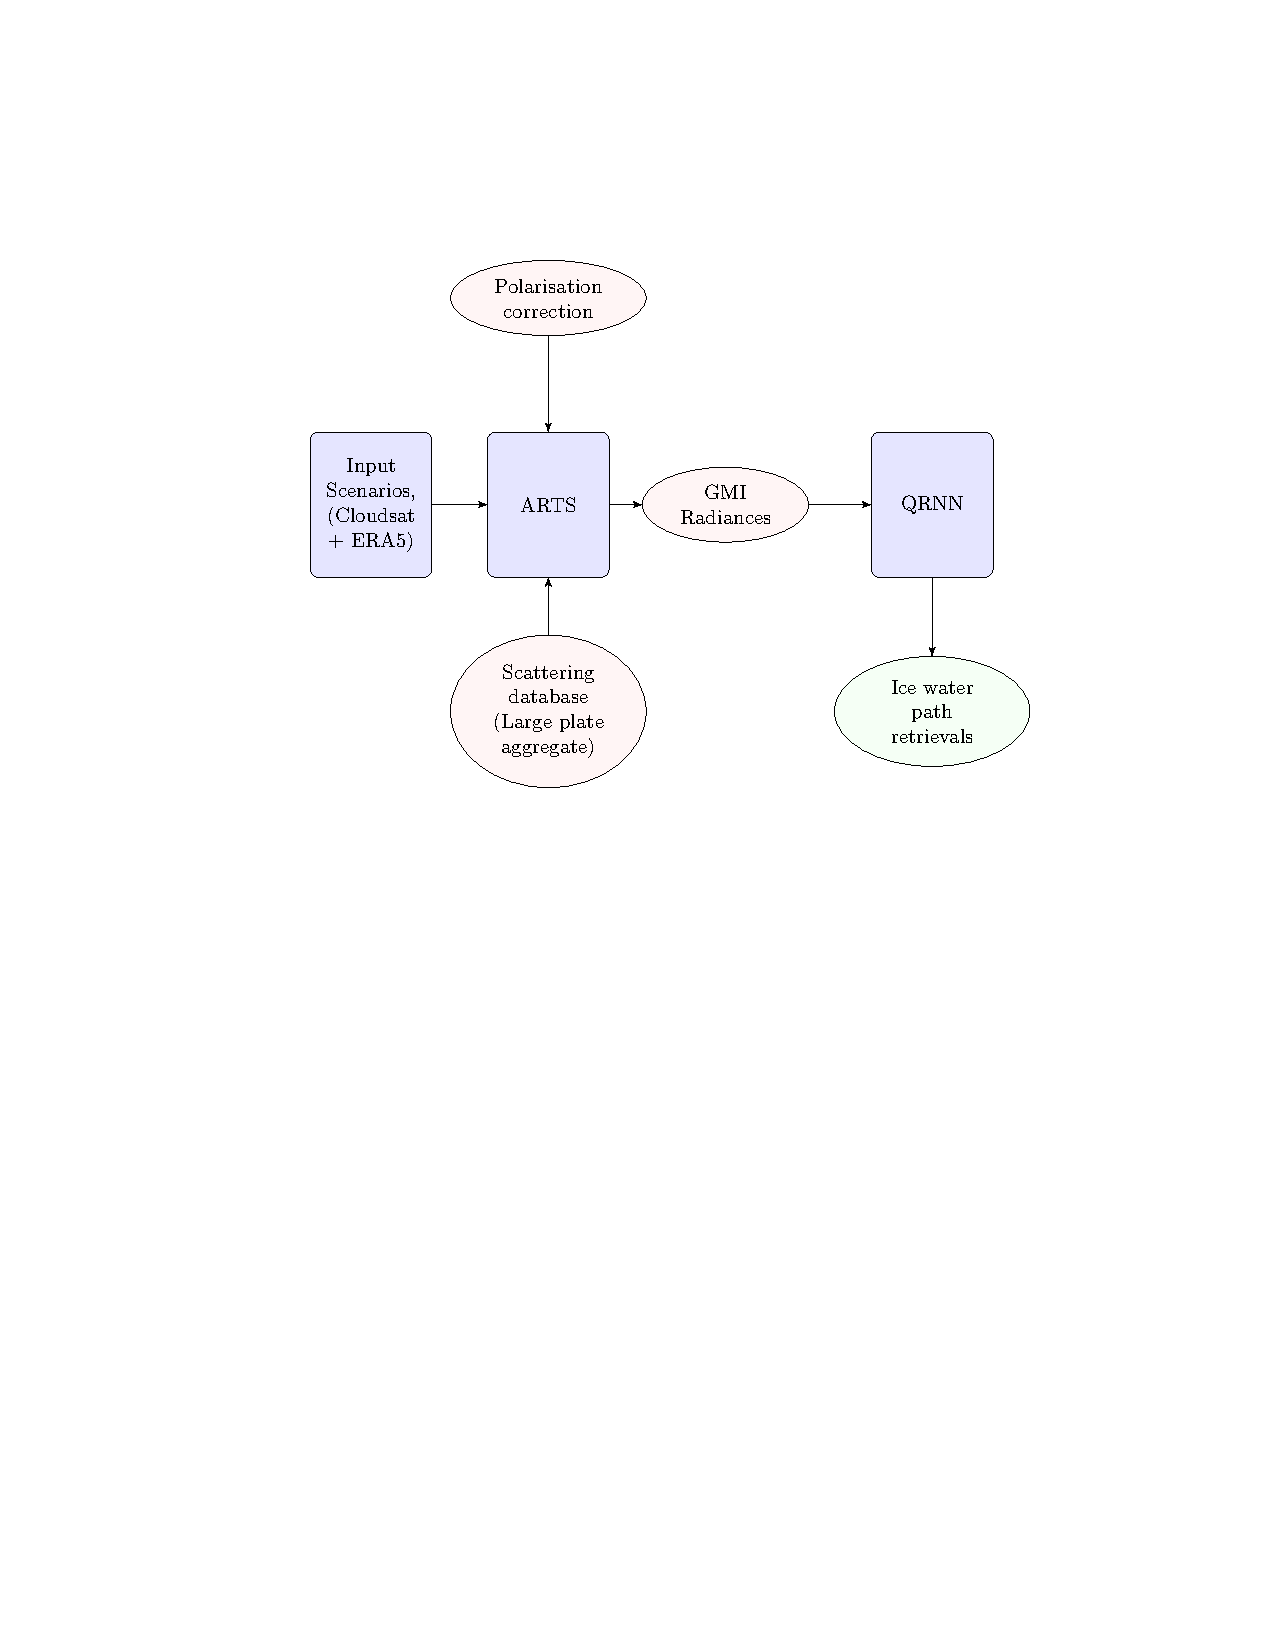
\includegraphics[trim=100 410 100 125,clip,height = 50mm, ]{Figures/flowchart.pdf}
	\caption{Flowchart showing the retrieval system.}
	\label{fig:flowchart}
\end{figure}

The main idea of this study is to combine a database based on radiative transfer with machine learning (ML) to retrieve IWP and the associated uncertainties. The ML algorithm (described below) uses the database to give the posterior knowledge of the quantity sought, given the scene of observations. Using ML on a retrieval database for to invert TB to IWP has advantages over the traditional inversion techniques. ML can avoid the uncertainties introduced by approximations. 

\subsubsection{QRNN}
\label{sec:QRNN}

The retrievals are based on a neural network based method called QRNN \citep{pfreundschuh:aneur:18}. QRNN is a neural network which learns to predict a vector of quantiles {$y_i$} representing the distribution of the output from a set of inputs {$x_i$}, through a series of learnable transformations. While training, the network seeks to minimise the model error through a quantile loss function. If $x_{\tau}$ is the $\tau$th quantile of a cumulative distribution function $F(X)$, the quantile loss function is defined as:

%\begin{equation}
%\mathcal{L}_\tau(y_\tau, y_{true}) =
%\begin{cases*}
%(1 - \tau)|y_\tau - y_{true}| &\text{if}  $y_\tau < y_\text{true}$\\
%\tau |y_\tau - y_\text{true}| & \text{ otherwise, }
%\end{cases*}
%\label{loss_function}
%\end{equation}

QRNN is available open source software quantnn \citep{} implemented with PyTorch backend \citep{paszke2017automatic}.


\subsubsection{QRNN inputs}

In order to implement an optimal QRNN for the current application, several factors were considered and are described in detail below. 

\begin{enumerate}
	
	\item  Firstly, it is crucial to define the best combination of input variables. The input vector space consists of TBs from the four high frequency channels of GMI ie., 166V\,\,GHz, 166H\,\,GHz, 183$\pm$3\,\,GHz, 183$\pm$7\,\,GHz. We also included 2\,\,m temperature, water vapour path, surface elevation and surface type as additional inputs to identify the environmental conditions. 
	
	\item The IWP has a very high dynamic range. A large majority of cases have very small or zero IWPs, but values as large at 25\,\,kg m$^{-2}$ also exist. Thus to facilitate the optimal use of data in the neural network, a loglinear transformation was applied. That is, all IWPs greater than 1.0\,\,kg m$^{-2}$  were transformed to natural logarithmic space, while the other IWPs remained unchanged. Additionally, all cases with IWP less 10$^{-4}$ were replaced by a small random number from the interval (10$^{-6}$, 10$^{-4}$).
	
	
	\item To avoid over-fitting a ML training model, data augmentation is often used to increase the variability in the data by adding noise. For our model, random noise was added to TB in each training cycle or epoch. The noise was added according to the NE$\Delta$T. 
	
	\item A small randomisation of the surface types was also included to take include misclassification in the database. Comparisons of the simulations and observations showed that GPROF surface classfication could be affected by misclassification. Thus to enhance the robustness of the machine learning model to these perturbations, the surface type of 1\% of the data was randomly shuffled at each epoch. 
	
%	\item QRNN was trained on approximately 900\,000 cases. The rest 200\,000 cases were used as validation dataset. The validation data is the part of the dataset which is used during the development of the training algorithm to quantify its performance. This dataset is different from the test data, on which the results are based on.	
	
	\end{enumerate}

\subsubsection{QRNN configuration}

	\begin{enumerate}	
		
	\item QRNN allows high resolution quantile fractions, and for this study, 51 equally spaced quantile fractions between 1\% and 99\% were selected. 	
	
	\item The multiple hyperparameters such as number of hidden layers, layer widths, batch size were selected by comparing the performance of the network over fixed set of values. The network architecture with lowest mean quantile loss was chosen for all QRNN trainings presented in this study. Finally, a neural network
	with five hidden layers and 256 neurons in each layer was selected. 
	
	\item \todo {SGD + cosine anealing. Start with lr = 0.01, train 20 epochs,  lower intial lr to 1e-4 and train for another 50 epochs, lr = 1e-5 and train for 100 epochs.}	
	
  
\end{enumerate}

 
\subsection{QRNN trainings}

To scrutinize the impact of databases on the retrieval performance, a separate QRNN is trained for each of the four databases : LPA-ARO, LPA-TRO, ESA-ARO, ESA-TRO (sect.~\ref{sec:database}). The basic construction of all trainings is identical (sect.~\ref{sec:QRNN}), except for the input retrieval database each is based on. 

Furthermore, two additional QRNN trainings are considered to monitor the impact of oriented hydrometeors. These two trainings are based on databases LPA-ARO and LPA-TRO, but the input data is slightly different. Here, instead of including both polarisation channels of 166\,\,GHz, only the V-polarised channel is included.

For each training, around 950\,000  simulations are used for training and around 200\,000 simulations are used for validation during the training. The validation data is the part of the dataset which is used during the development of the training algorithm to quantify its performance. This dataset is different from the test data, on which the results are based on. Additionally, another set of LPA-ARO simulations consisting of 100\,000 cases is used as a test dataset to evaluate the  basic retrieval performance. These simulations are not revealed to QRNN during training. 


\subsection{Evaluation}
\label{sec:evaluation}

Conventional retrieval methods provide single point estimates, but QRNN retrieves the posterior distribution in terms of quantiles. The quantiles quantify the preduction uncertainty through a probabilistic upper and lower bound for each case. For evaluating the retrieval accuarcy, we select the expectation value $\mathbb{E}(y)$ as the point estimate. 





\section{Results}

\subsection{Polarisation ratio}
\label{sec:polratio}
\begin{figure*}[t]
	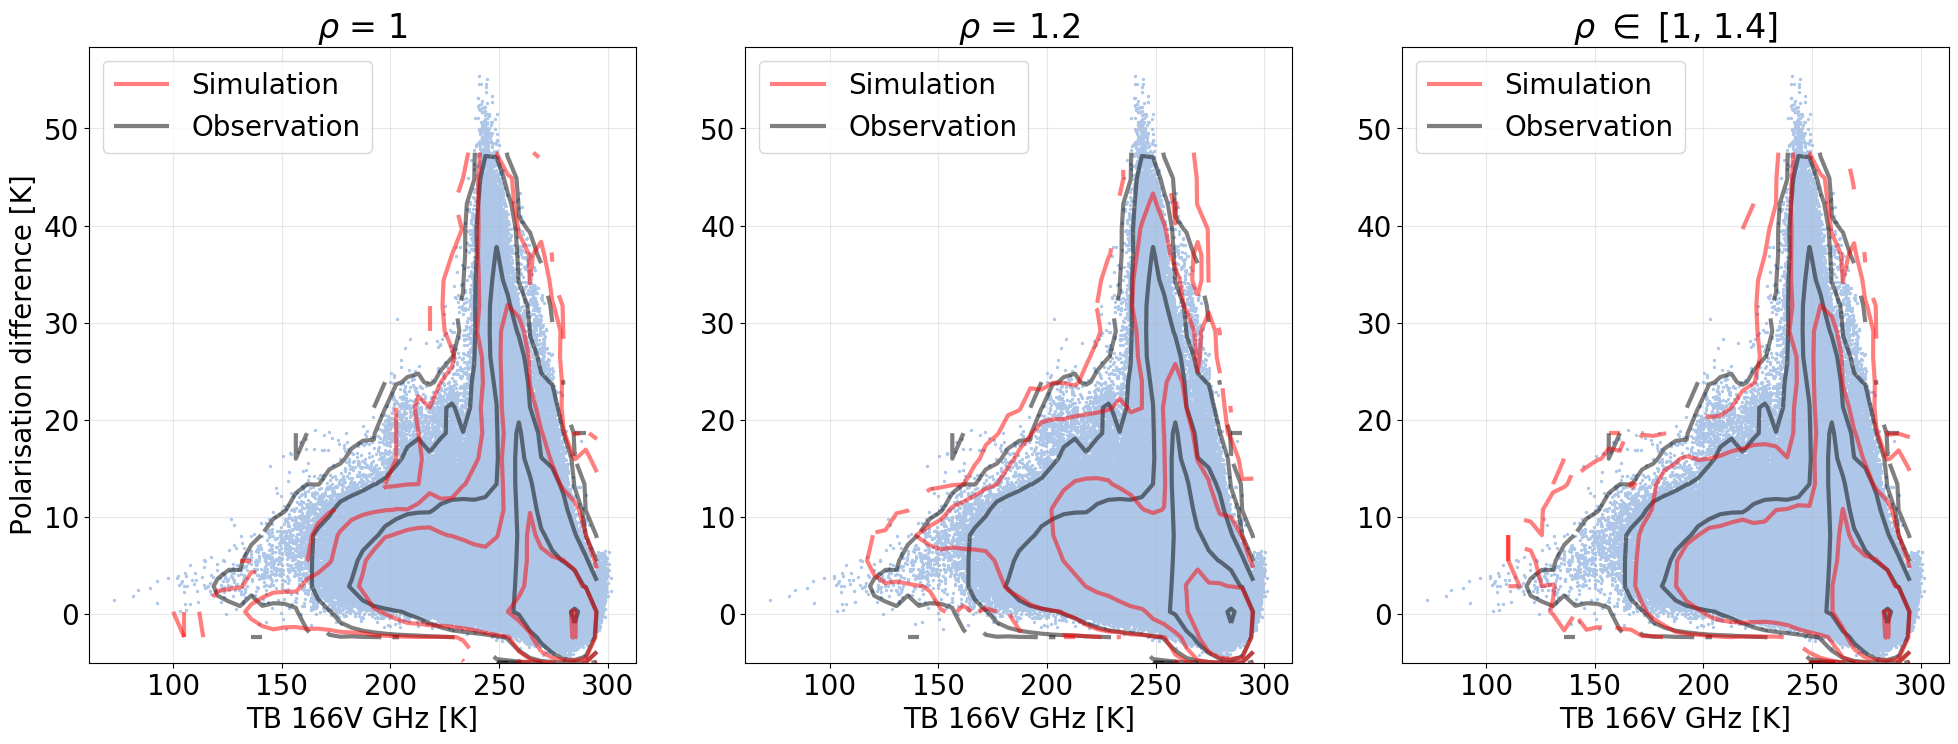
\includegraphics[width=8.3cm]{Figures/PD_166.png}
	\caption{The polarisation differences (166V - 166H) as a function of
		brightness temperatures at 166V GHz ( PD-TB$_V$ relationship) for observations (black) and simulated (red) for dfferent values of $\rho$. The scatter plot from the observations is also plotted in light blue.}
	\label{fig:PD_166}
\end{figure*}
\begin{figure}[t]
	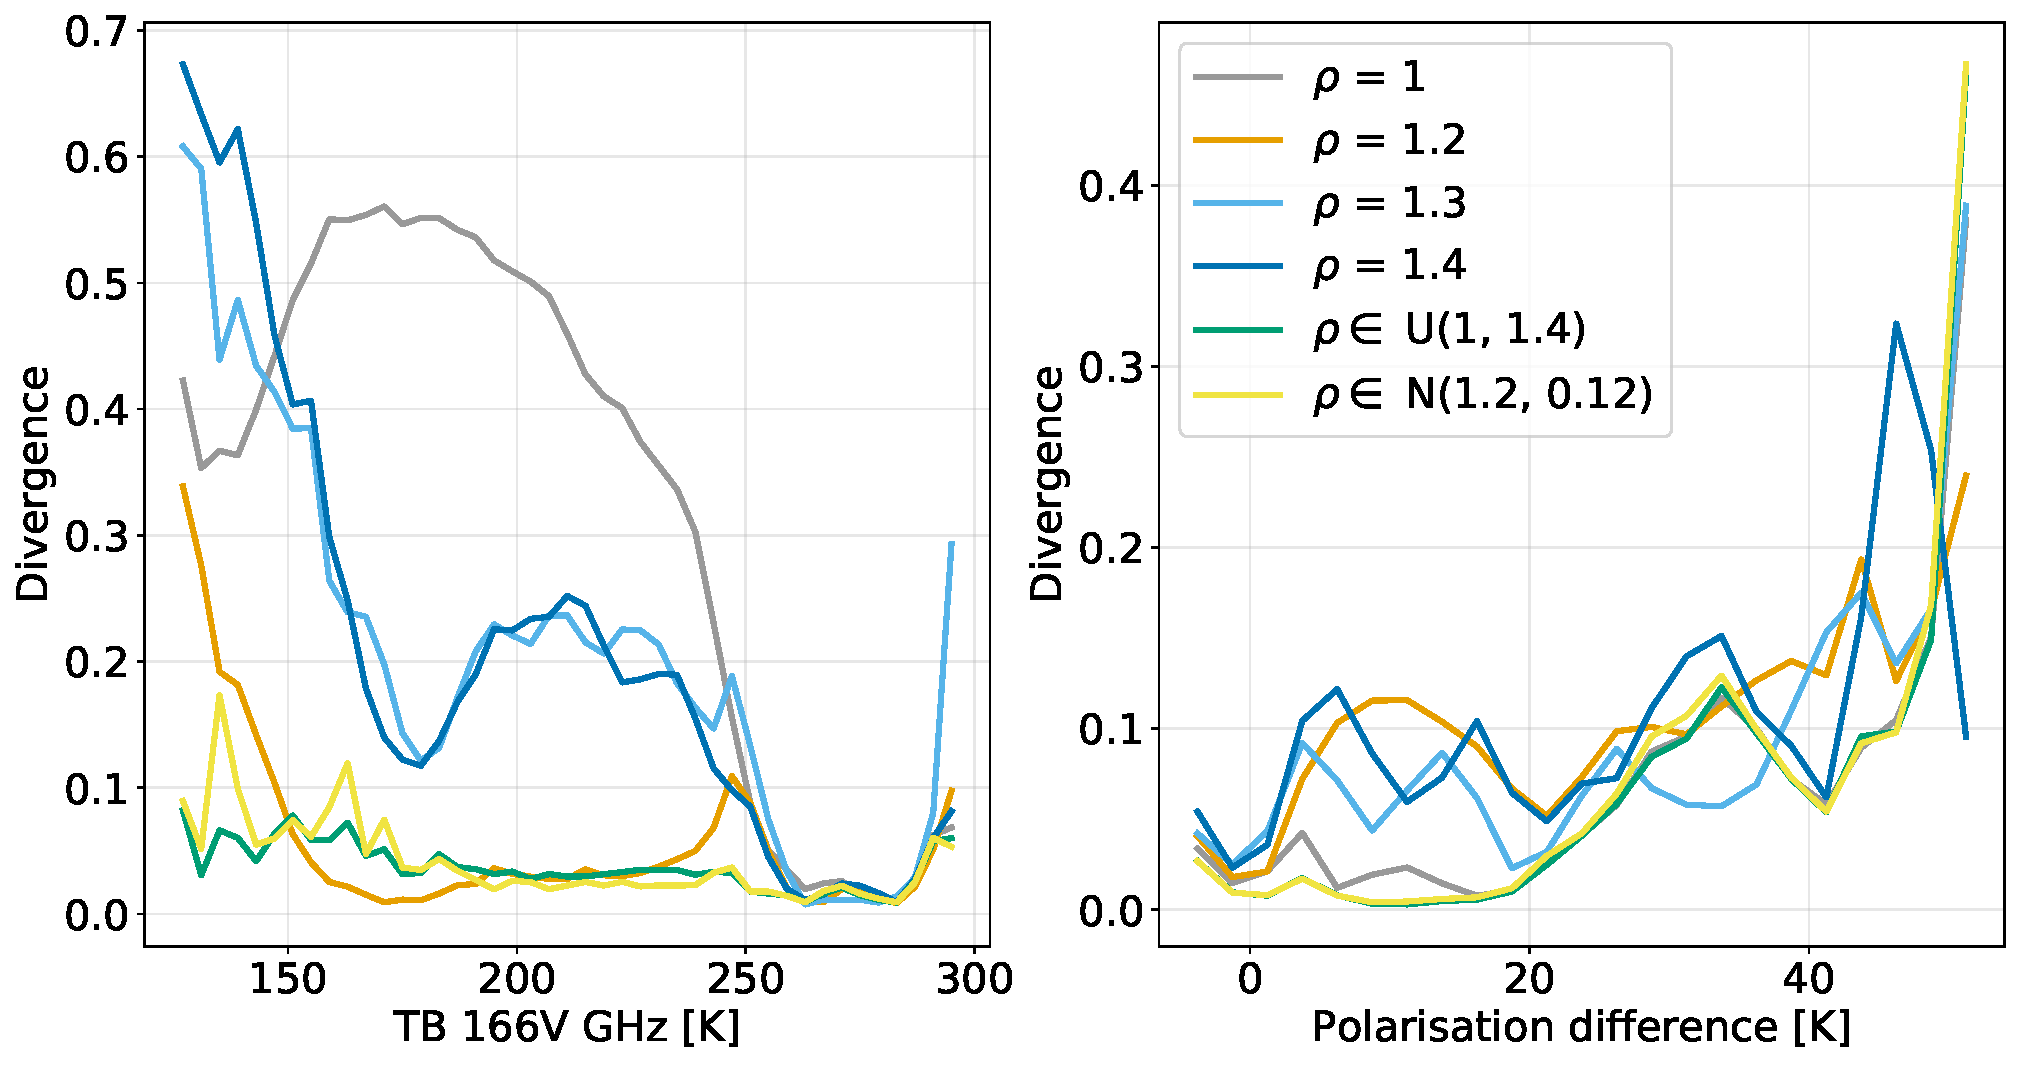
\includegraphics[width=8.3cm]{Figures/divergence.pdf}
	\caption{The J-S divergence describing the differences between the two-dimensional PD-TB$_V$ relationship between observations and simulations along (a) TB axis and (b) PD axis. Results from the four experiments with different values of $\rho$ are shown. }
	\label{fig:divergence_PD}
\end{figure}

The preferential orientation of the ice hydrometeors has a larger impact on the scattering effects than randomly oriented particles. The scattering affects the TB depression and contributes towards enhancing the difference between V- and H- polarised channels \citep{xie:polar:11}
The PD have a very unique relationship with TB. Figure~\ref{fig:PD_166} shows the PD-TB$_V$ relationship observed at 166\,\,GHz. Polarisation signals introduced by both surface contribution and hydrometeor scattering are are included in this figure. The contribution from oriented ice particles is mostly concentrated below 250\,\,K and they follow a arch shape curve. On the other hand, the large PDs concentrated along the arm are introduced by scattering from the surface, especially over water. The magnitude of maximum PD can vary with frequency or on the surface type it was measured, but \citet{gong:micro:17} have shown that this arch or bell shape pattern appears universally at all high microwave frequencies. We describe these PDs in detail in Sect.~\ref{sec:PD} 

In this study, we utilize the PD-TB$_V$ relationship at 166\,\,GHz to select the value of $\rho$ providing the best fit between simulations and observations. The simulations do not have a one-to-one correspondence with the observations, but are expected to have a similar statistical distribution. In order to quantify the measure of similarity between the observed and simulated PD-TB$_V$ distributions, we employ the Jensen–Shannon divergence method \citep{}. This method calculates the divergence between the true and the approximated distribution. It is a symmetric and smooth implementation of the Kullback–Leibler divergence \citep{}. If $P^o$ and $P$ are two probability distributions and $KL (P^o \parallel P)$ denotes the Kullback–Leibler divergence between the two, then J-S divergence is defined as:

\begin{equation}
JSD(P^o \parallel P) = 0.5 \times (D(P^o \parallel R)+D(P \parallel R))
\end{equation}

where, $R = 0.5 \times (P^o + P)$ is the mid-point of the probability vectors $P^o$ and $P$. $JSD$ can take values between $[0, \inf]$, where small values indicate low divergence. $JSD$ is equal to zero only if $P^o$ and $P$ are identical distributions. For two-dimensional distributions, the divergence can be calculated along both dimensions.   


To model the effects of $\rho$ five experiments with identical set-up but different values of $\rho$ are conducted. In first three experiments, forward modelled radiances from January 2009 are estimated for $\rho = 1, 1.2, 1.3$. In the fourth experiment, $\rho$ is selected randomly from a truncated normal distribution with mean = 1.2, and standard deviation .... In the fifth experiment, a uniform distribution for $\rho\in[1, 1.4]$ is assumed. 
%The input atmospheric scenarios are identical in each experiment. 

Figure~\ref{fig:PD_166} shows the PD-TB$_V$ relationship for different values of $\rho$. The region of high interest with respect to this study is the arch like structure, which originates from the cloud ice scattering. When all hydrometeors are assumed to be TRO ($\rho = 1$), simulations are unable to capture the PDs observed for colder radiances. Below 200\,\,K the simulated PDs start to flatten out. Nonetheless, the surface contributions match quite well. In the second experiment, when all cases are scaled by $\rho = 1.2$, the very low PDs (below 2\,K) from hydrometeor scattering are absent and the PDs > 5\,K are over-represented. Similar is the case in the third experiment with $\rho = 1.4$. In this case the over-representation is further increased. In all three experiments, the surface impact remains unchanged, and matches well with observed distribution. Figure~\ref{fig:divergence_PD} displays the J-S divergences along both dimensions (TB and PD) for all four experiments. For the first three experiments, the match between the distributions is quite high for towards the warmer radiances, i.e. surface impact. This is in line with the results seen in the two-dimensional histograms. Towards the colder radiances (< 175\,\,K), the divergence is lowest for $\rho = 1.2$, and maximum for $\rho = 1$. But between 175\,\,K and 250\,\,K, $\rho = 1.2$ has the highest mismatch. Increasing the polarisation ratio helps in reducing the differences for the colder radiances but at the cost of over-representation. Similar behaviour is also observed for $\rho = 1.4$.
THe fourth experiment however behaves differently. With a variable $\rho$ the simulated PDs both induced by clouds and as well as the surface contribution well approximated. The divergence for this set-up is lowest among all four experiments, particularly for the range 150 - 250\,\,K where most cloud induced PD are observed. 

The results from these four experiments show that a single value of $\rho$ is not sufficient to mimic a realistic PD distribution. While inclusion of ARO particles is important, effect from TRO cannot be completely ignored. In reality, the polarisation patterns depend on the microphysical properties, and the complex mixture of hydrometeors in the atmosphere can generate a plethora of polarisation signals. This wide spectrum of polarisation signals cannot be reproduced correctly by constraining the particle model to only one habit and size distribution, and one polarisation ratio. In this study, since we accomodate only one particle model, choosing a constant $\rho$ constrains the PDs to a narrow range. A random selection of $\rho$ can alleviate this limitation to a certain extent. Based on the results from the four experiments described above, we select $\rho$ from a uniform distribution between [1, 1.4].

\subsection{Comparison of simulations and measurements}

\subsubsection{TB distribution}

\begin{figure}[t]
	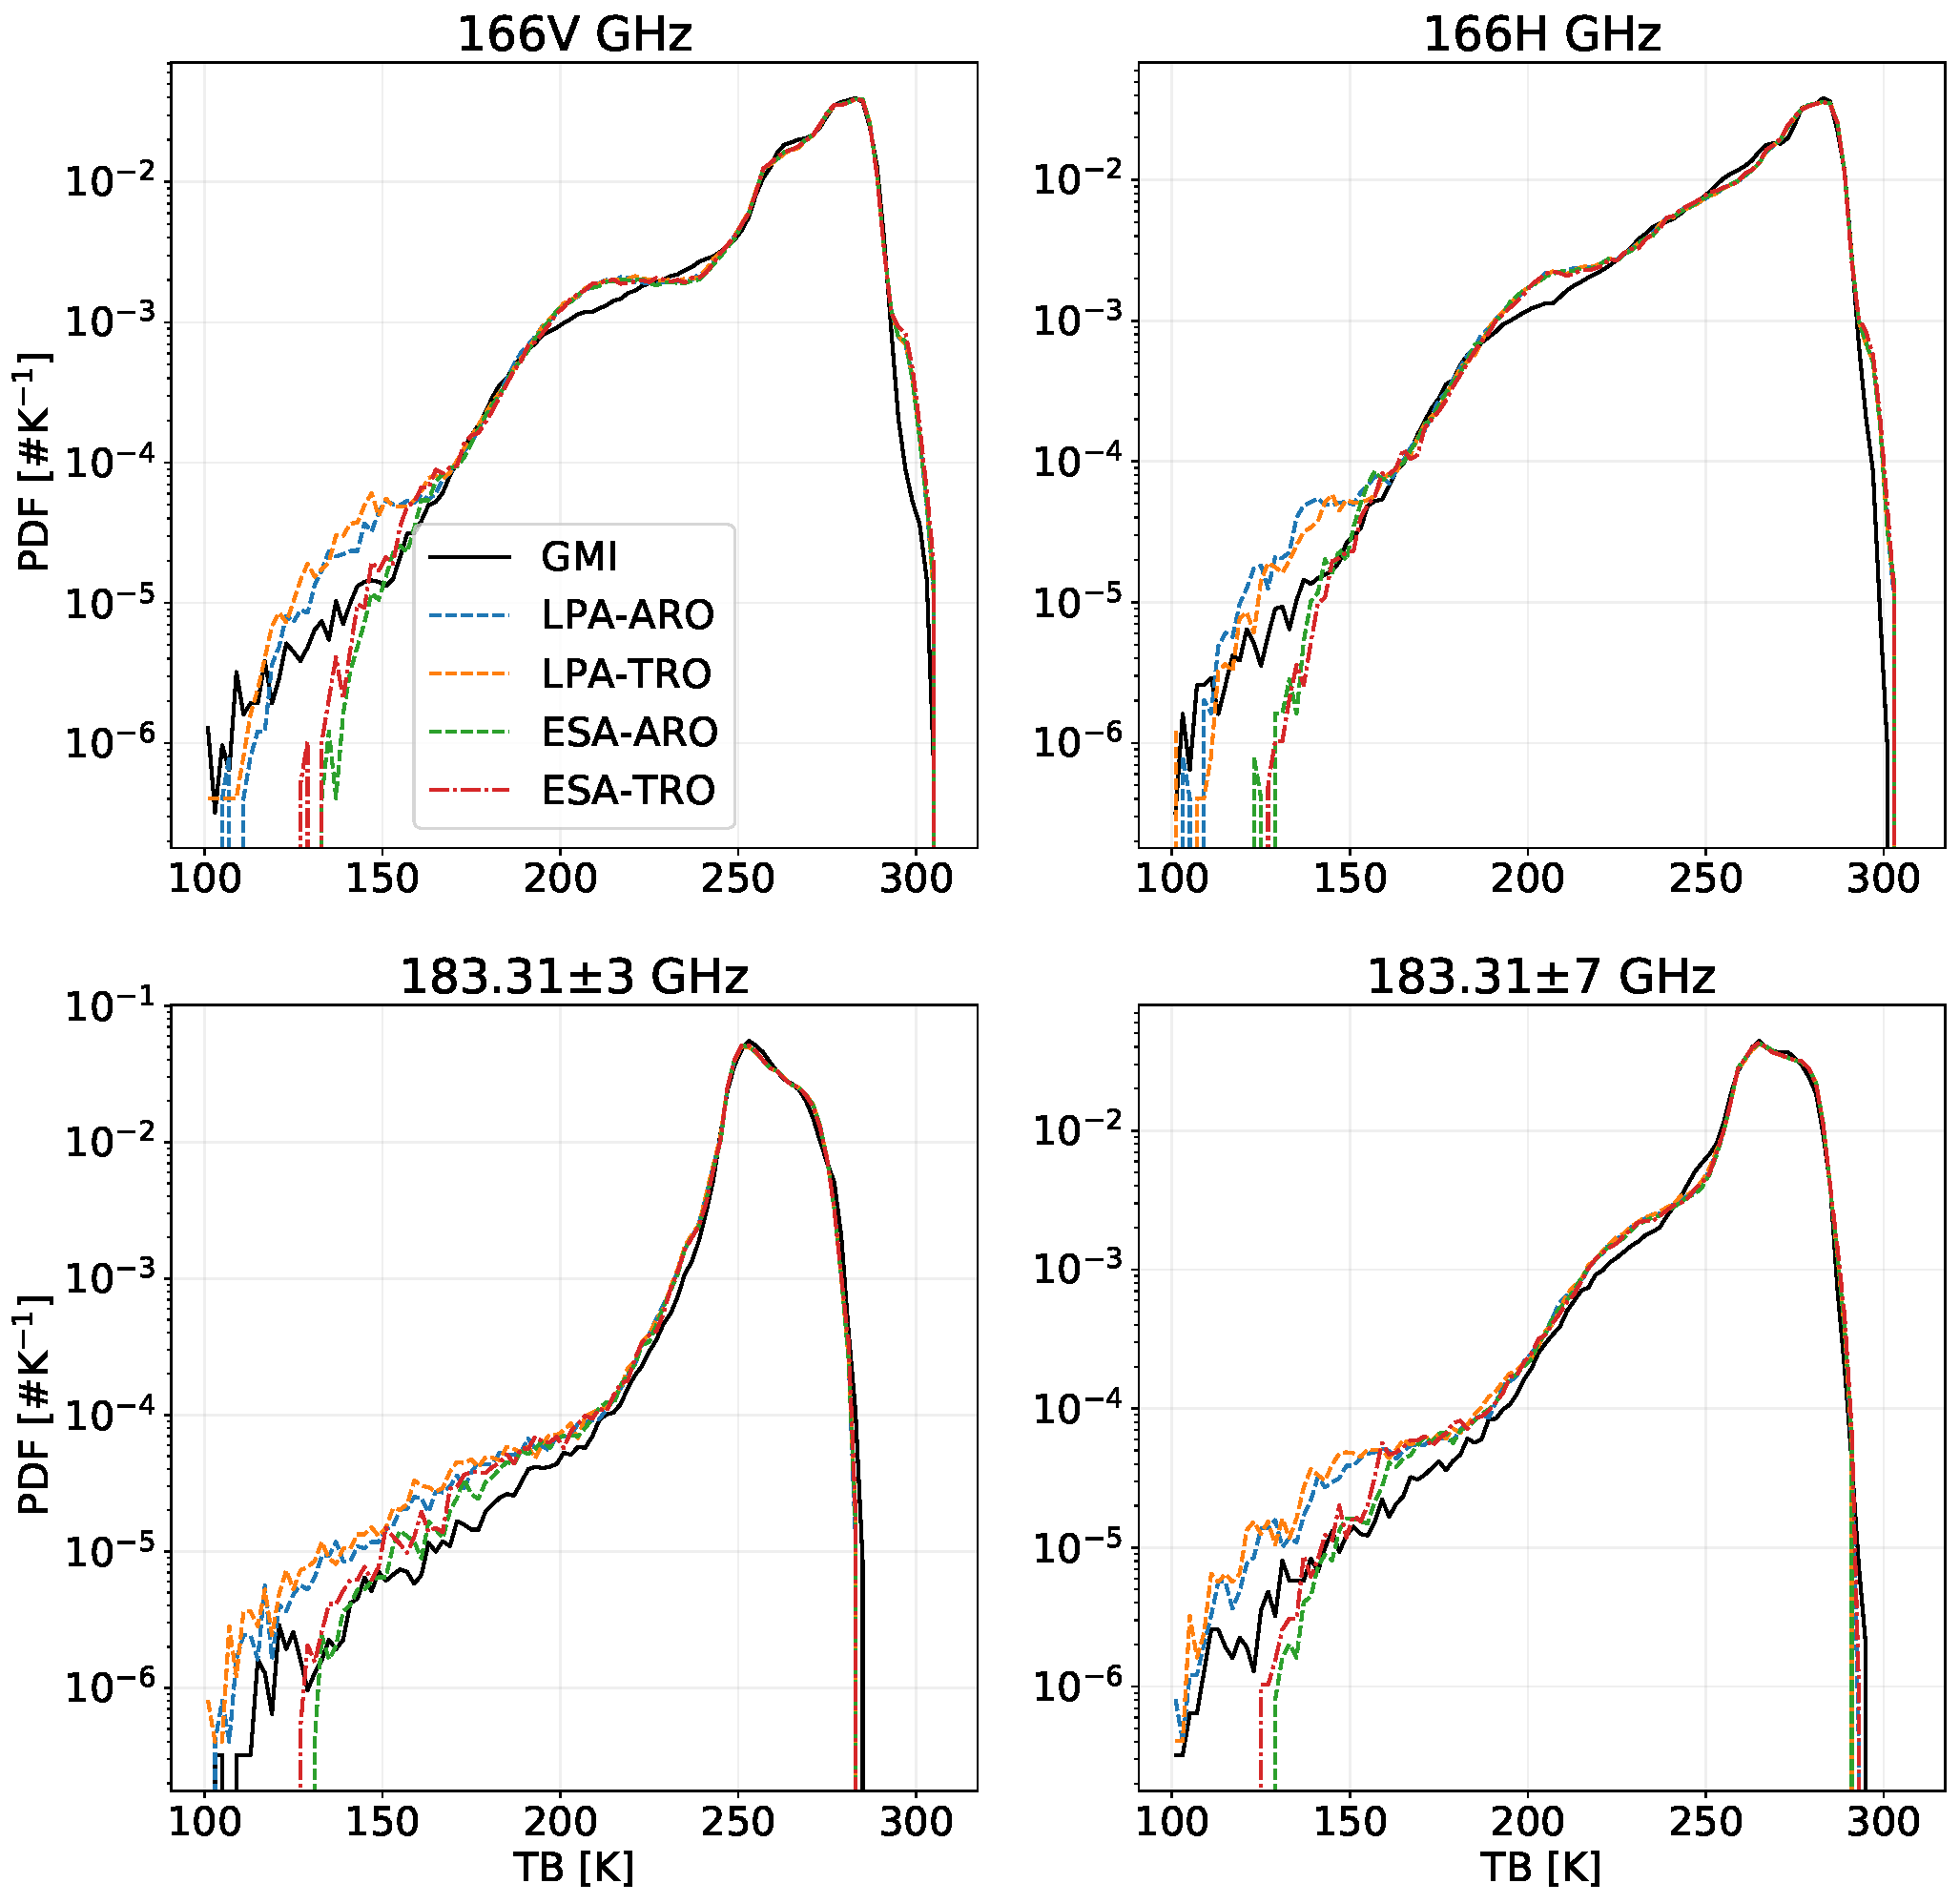
\includegraphics[width=8.3cm]{Figures/PDF_TB_jan.pdf}
	\caption{Distribution of TBs for all high frequency channels of GMI . The black curve represents the GMI measurements, while the four curves denote the four simulation databases.}
	\label{fig:hist_TB}
\end{figure}

This section describes the performance of simulated TBs for all four high frequency channels of GMI. The simulated values are based on random Cloudsat profiles thus only a statistical comparison with the observations is made. It is not necessary for the simulations to be collocated with the GMI observations in space and time, but a similar variability between the two is expected. For retrieval to be successful, the database should reflect the realistic scenarios. 

%A comparison of the mean TB difference is also made in Table~\ref{tab:mean_TB}. The mean TB   is calculated as

Figure~\ref{fig:hist_TB} shows the distribution of simulated TBs for each channel and all four databases (see sect.~\ref{sec:database}). The distribution of GMI observations is also plotted in black. For all four channels, the peak of the distributions correspond to the clear-sky scenarios, while the coldest TBs are associated with deep convective systems. For clear-sky cases, all four databases agree well with GMI.

However, over the colder part of the TBs none of the four databases are able to reproduce the exact distribution. With large plate aggregate, the forward simulations put more cases with low TBs, while with evans snow aggregate, the model falls short of simulating the coldest TBs. At the intermediate region (between 170\,\,K and 250\,\,K) the simulations have a high occurrence frequency for all channels except 183$\pm$3. Analysing the distributions according to surface type and latitudinal extent revealed that the mismatch is removed when TBs over snow surface type are not included (not shown). Indicating that the forward simulations have a larger representation of snow cases than GMI. Since snow cover is a variable quantity, a comparison between data from different time scales can introduce such artefacts. 

Inclusion of ARO particles has a small impact on occurence frequency of colder TBs. With both habits, when only TRO particles are simulated, the deep convection zone has a higher frequency of colder TBs. But when ARO particles are included, a drop in frequency indicates that slighly warmer TBs are simulated. 

The comparison of GMI observations and simulations shows that an overall agreement is fairly good. The main differences exist towards the colder brightness temperatures which reflect the deep convections systems. The mismatch is higher as only one habit and PSD are considered in each database. However, both particle habits have a very different behaviour towards the convective end. Large plate aggregate result in larger TB depressions than evans snow aggregate. The effect can be explained by the interaction of particles with electromagnetic radiation. Under the assumed PSD, F07T, the larger ice particles introduce higher scattering for increasing values of IWC, and for lower IWC, the impact of intermediate size particle (effective diameter ~ 0.5\,\,mm) dominates. While this is a general behaviour, the exact scattering impact depends on the mass-size relationship of the particle model. Thus for the convective zone where IWC are higher, notabale differences are osberved between the two particle models. Large plate aggregate, which has larger cloud ice particles, puts colder TBs in the convective zone in comparison to evans snow aggregate. However, for the intermediate zone, where contribution from liquid particles dominates, the two particles models produce comparable TBs.

Further, the TBs in the ARO based databases are slightly warmer towards the convective end. \todo{incomplete}

\subsubsection{Polarisation differences}
\label{sec:PD}

\begin{figure}[t]
	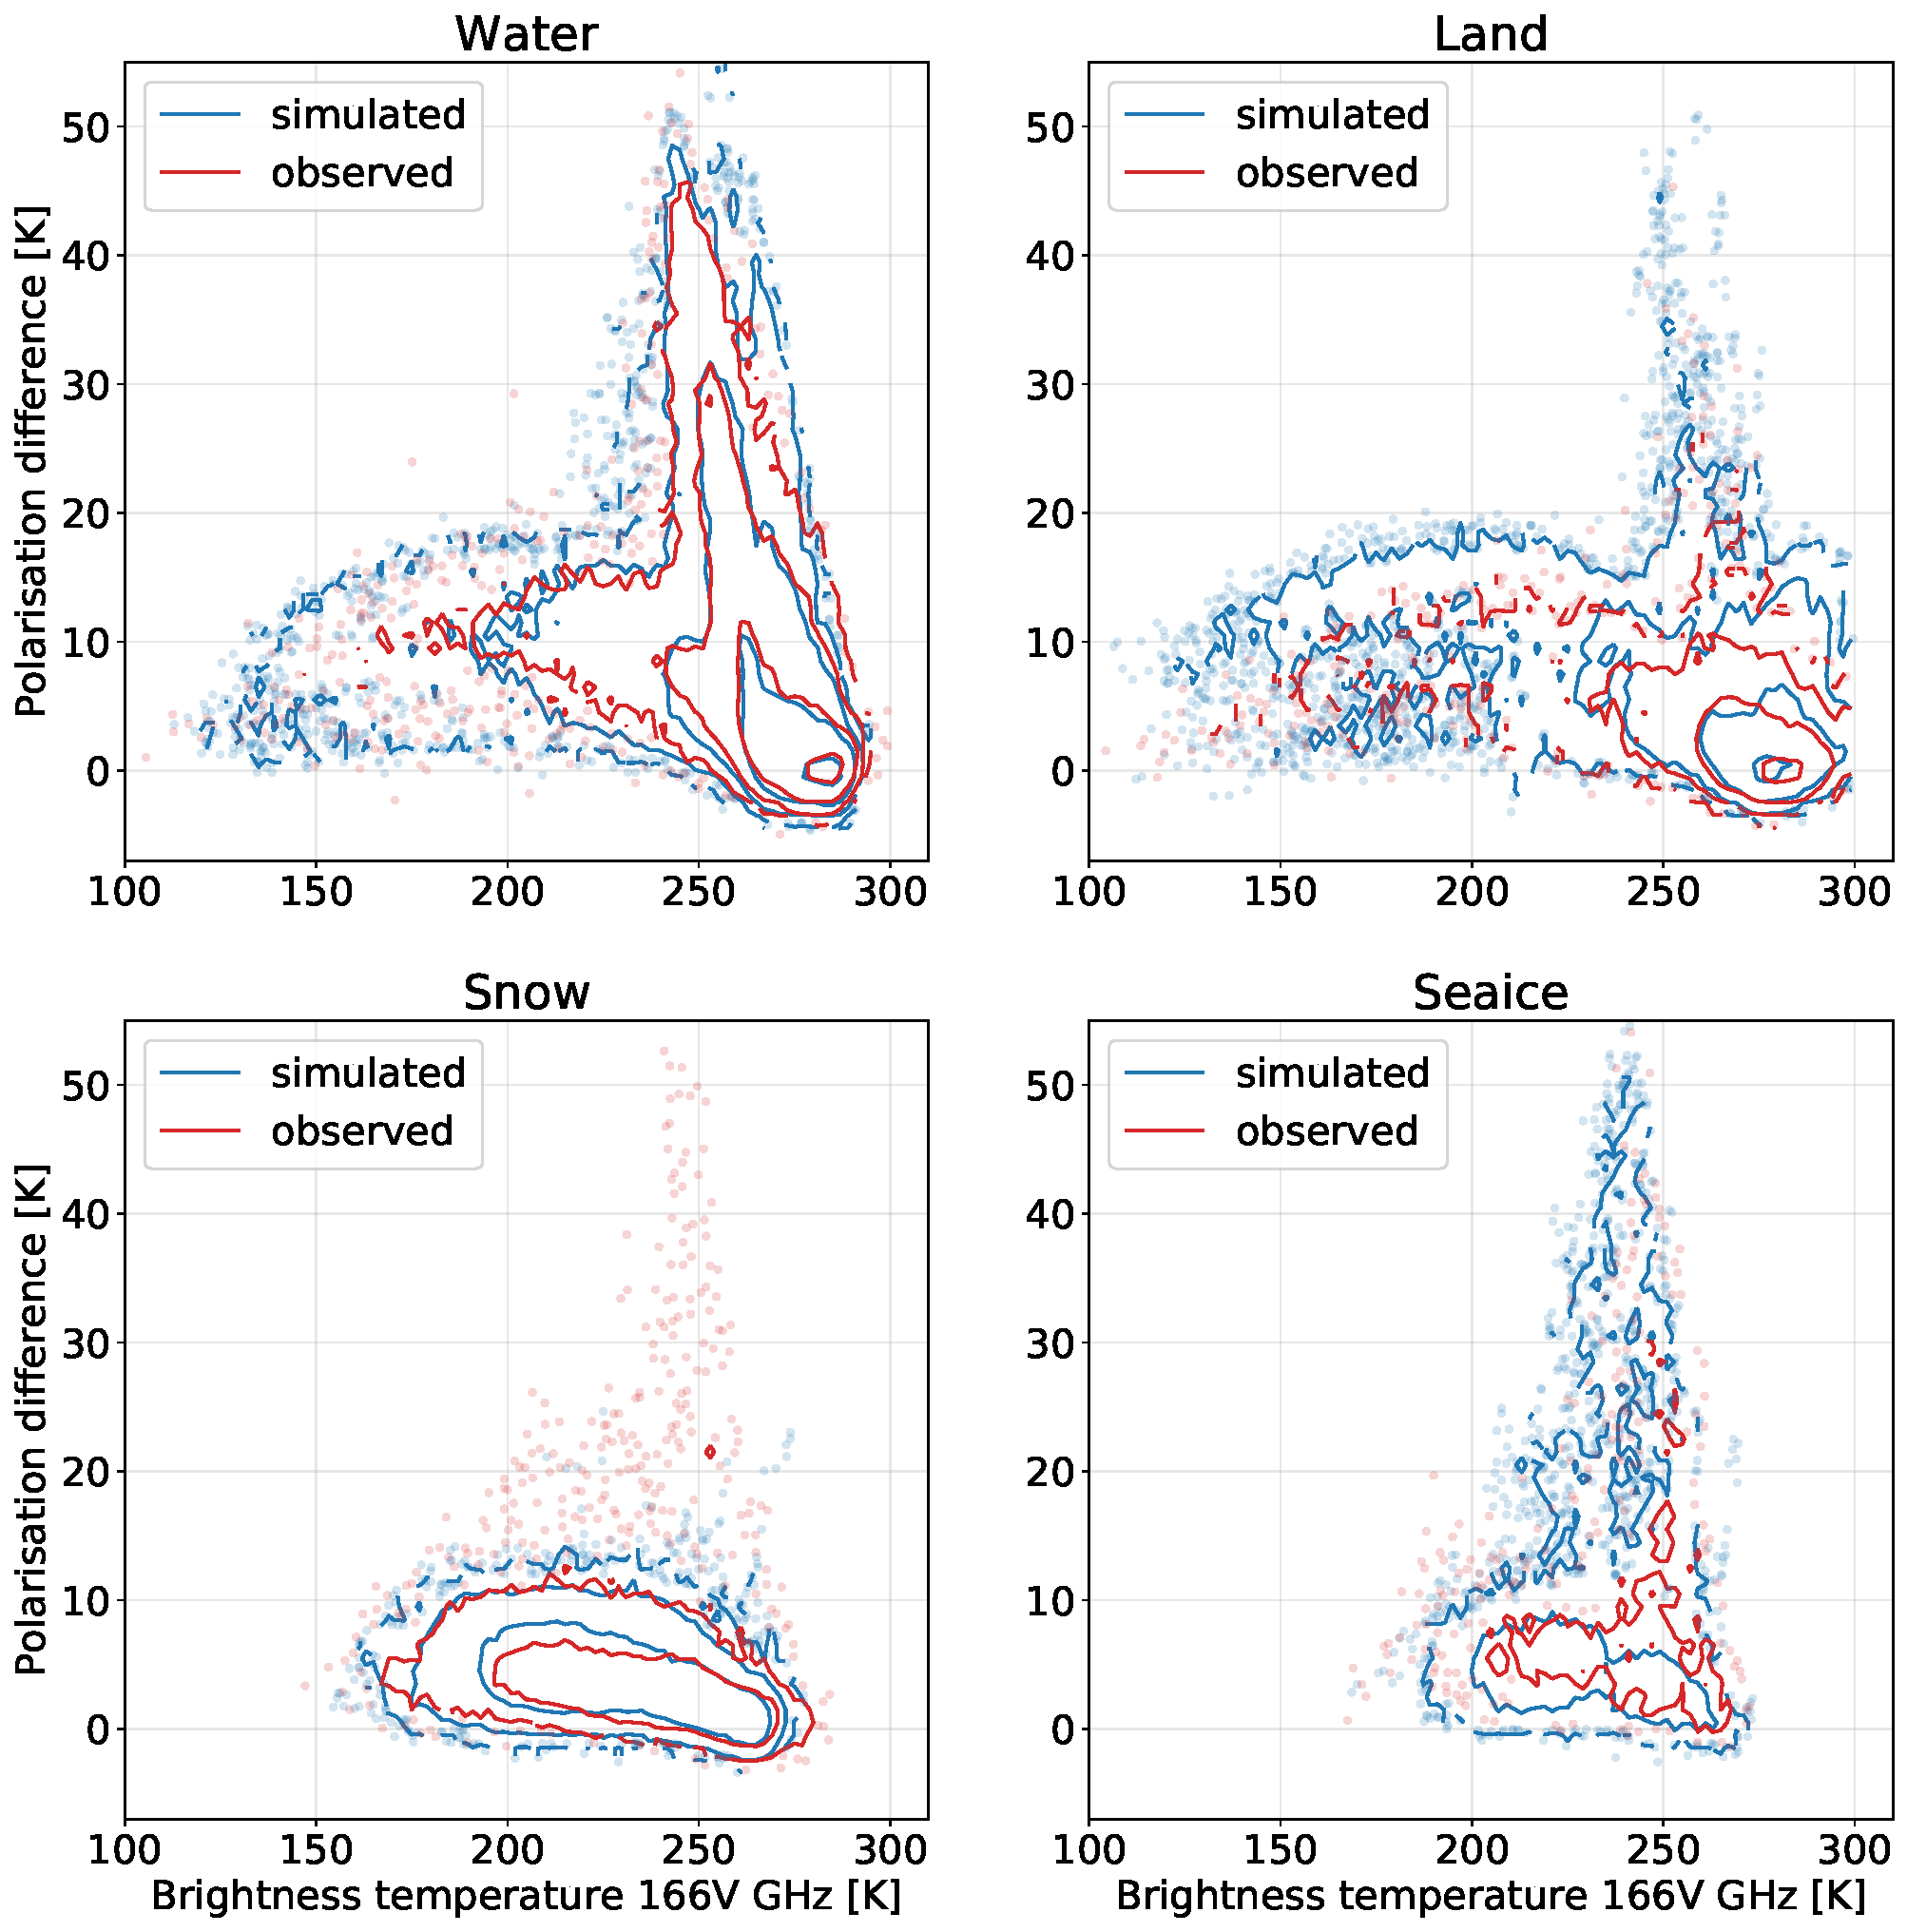
\includegraphics[width=8.3cm]{Figures/hist2d_all_surface_jan.pdf}
	\caption{Polarisation differences (166V - 166H) as a function of
		TB 166V GHz for observed (red) and simulated (blue) for
		different surface types.}
	\label{fig:PD}
\end{figure}

This section provides a more thorough description of the PDs.  Figure~\ref{fig:PD} shows the observed and simulated PDs categorised by the surface type. PDs from both surface contribution and hydrometeor scattering are included. For all four surface types, the TB-PD relationship is characterised by a strong arm consisting of very high PDs centered around 250\,\,K and a cluster of cases forming a arch like structure. The arch is stronger over land and water than snow and seaice. 

The strong vertical arm is due to TB depressions introduced by surface scattering. The strongest PD are observed over land and water under dry atmospheric conditions. In the presence of water vapour, the signal from the surface is attenuated and the PDs cluster around the bottom tip of the distribution. For snow and seaice the vertical arm is weak. It mostly consists of contribution from mixed surface types : snow/land boundary and seaice/water boundary respectively. 

As earlier mentioned, we are highly interested in the arch region, where maximum impact of ice hydrometeors lies. For land and water the arch is quite strong. For these surface types, maximum PD are centered around 200\,\,K. The PDs diminish towards the colder TBs, while towards the warmer end, the PDs from clear-sky overlap. 


However, over snow and seaice due to high surface impact, the flat cluster of PDs are a mixture of surface and hydrometeor contribution.
 


\subsection{IWP retrievals}
%
\subsubsection{Basic retrieval performance}
%
\label{sec:basic_performance}

\begin{figure}[t]
	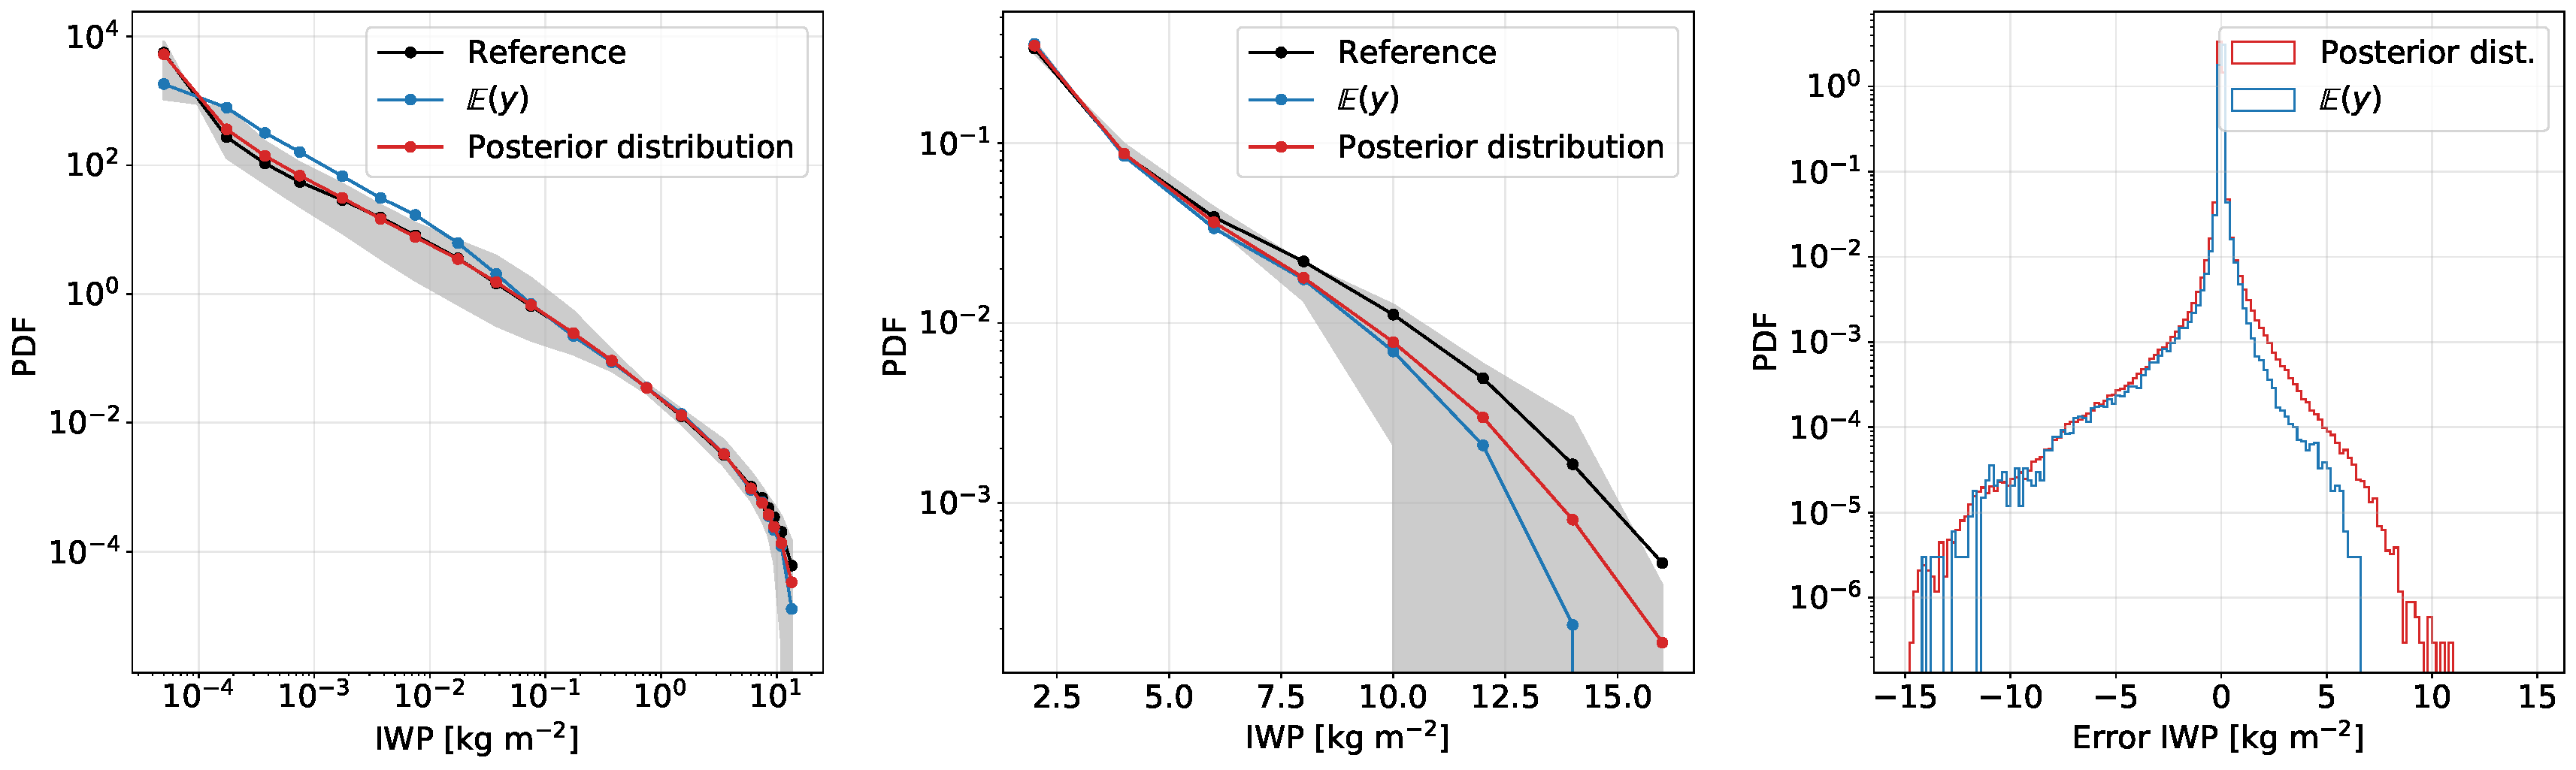
\includegraphics[width=8.3cm]{Figures/PDF_IWP_ARO.pdf}
	\caption{}
	\label{fig:PDF_IWP_test}
\end{figure}

To evaluate the  retrieval performance of QRNN, the training based on LPA-ARO is applied on the test dataset. This dataset is part of the LPA-ARO database, but not revealed to the network during training. It provides a way to check the model accuracy against the data that was not used in the training procedure. We retrieve the IWPs for the test dataset and compare against the true state vectors. This is a idealised retrieval where both the training and test datasets have same underlying a priori distributions. As mentioned in sect.~\ref{sec:evaluation} the expectation value is taken as the point estimate. It is referred as retrieved IWP henceforth. 

Figure~\ref{fig:PDF_IWP_test}(a) shows the normalised distributions of the observed and retrieved state vectors. The posterior distribution and the spread of the retrievals in the 94\% confidence interval are also shown. The posterior distribution agrees quite well with the truth, but the expectation value has a different behaviour. For low IWPs (< 0.01\,\,kg m$^{-2}$) the occurence frequency of retrieved IWPs is higher, while the very high IWPs (> 10\,\,kg m$^{-2}$) occur less frequently. For IWP greater than 0.1\,\,kg m$^{-2}$, the dispersion in the 94\% confidence interval is quite low, thus the retrievals are  sharper and better calibrated. However, for very low IWPs, the retrieved IWPs lie outside the 94\% confidence interval and are poorly calibrated. In this case, while using the median value might give a better retrieval accuracy, but the expectation value is a bias free estimate. 

\todo{ask Simon for more input here}
 
Overall, QRNN overestimates the low IWP values (thin ice clouds) and  slightly underestimates the larger IWPs (thick ice clouds). 


Figure~\ref{fig:PDF_IWP_test}(b) shows the MFE between the retrieved and reference IWP. For IWP < 0.01\,\,kg m$^{-2}$, the MFE is larger than 200\%, but for IWP > 0.1\,\,kg m$^{-2}$ it drops rapidly from 100\% to almost 20\%. 

\todo{compare MFE values with Brath ISMAR  and SpareIce?}

  

\subsubsection{Impact of oriented particles}
%
To examine the impact of oriented hydrometeors in IWP retrieval, we compare the results from LPA-ARO and LPA-TRO based training. Although, LPA-TRO has a different a priori distribution than LPA-ARO, for an exact comparison, we use an identical test data (based on LPA-ARO). In this case, the retrievals based on LPA-TRO training will not reflect the true QRNN performance, but the same is also not expected. In ideal world, a trained model is expected to make predictions using input data following the same underlying distributions, however for realistic situations this assumption can be violated due to many aspects not considered in the database. Similar is the situation with LPA-TRO database. This database lacks the contribution from oriented hydrometeors, but in reality, this effect is quite important. Basing the comparison of LPA-ARO and LPA-TRO based trainings on a LPA-ARO test dataset, can quantify the IWP errors introduced by neglecting polarised signals. The retrievals based on these trainings are denoted by the name of the database they trained on.

Two types of comparisons are made. Firstly, a comparison of the retrievals based on QRNN trained with both V and H polarised channels  is made. Secondly, a comparison of retrievals based on QRNN trained with only V- polarised channel is made. The retrievals from these two trainings are referred as LPA-ARO(V) and LPA-TRO(V) further in the text.  

\paragraph{Including both V and H}
\label{sec:results_vh}

\begin{figure*}[t]
	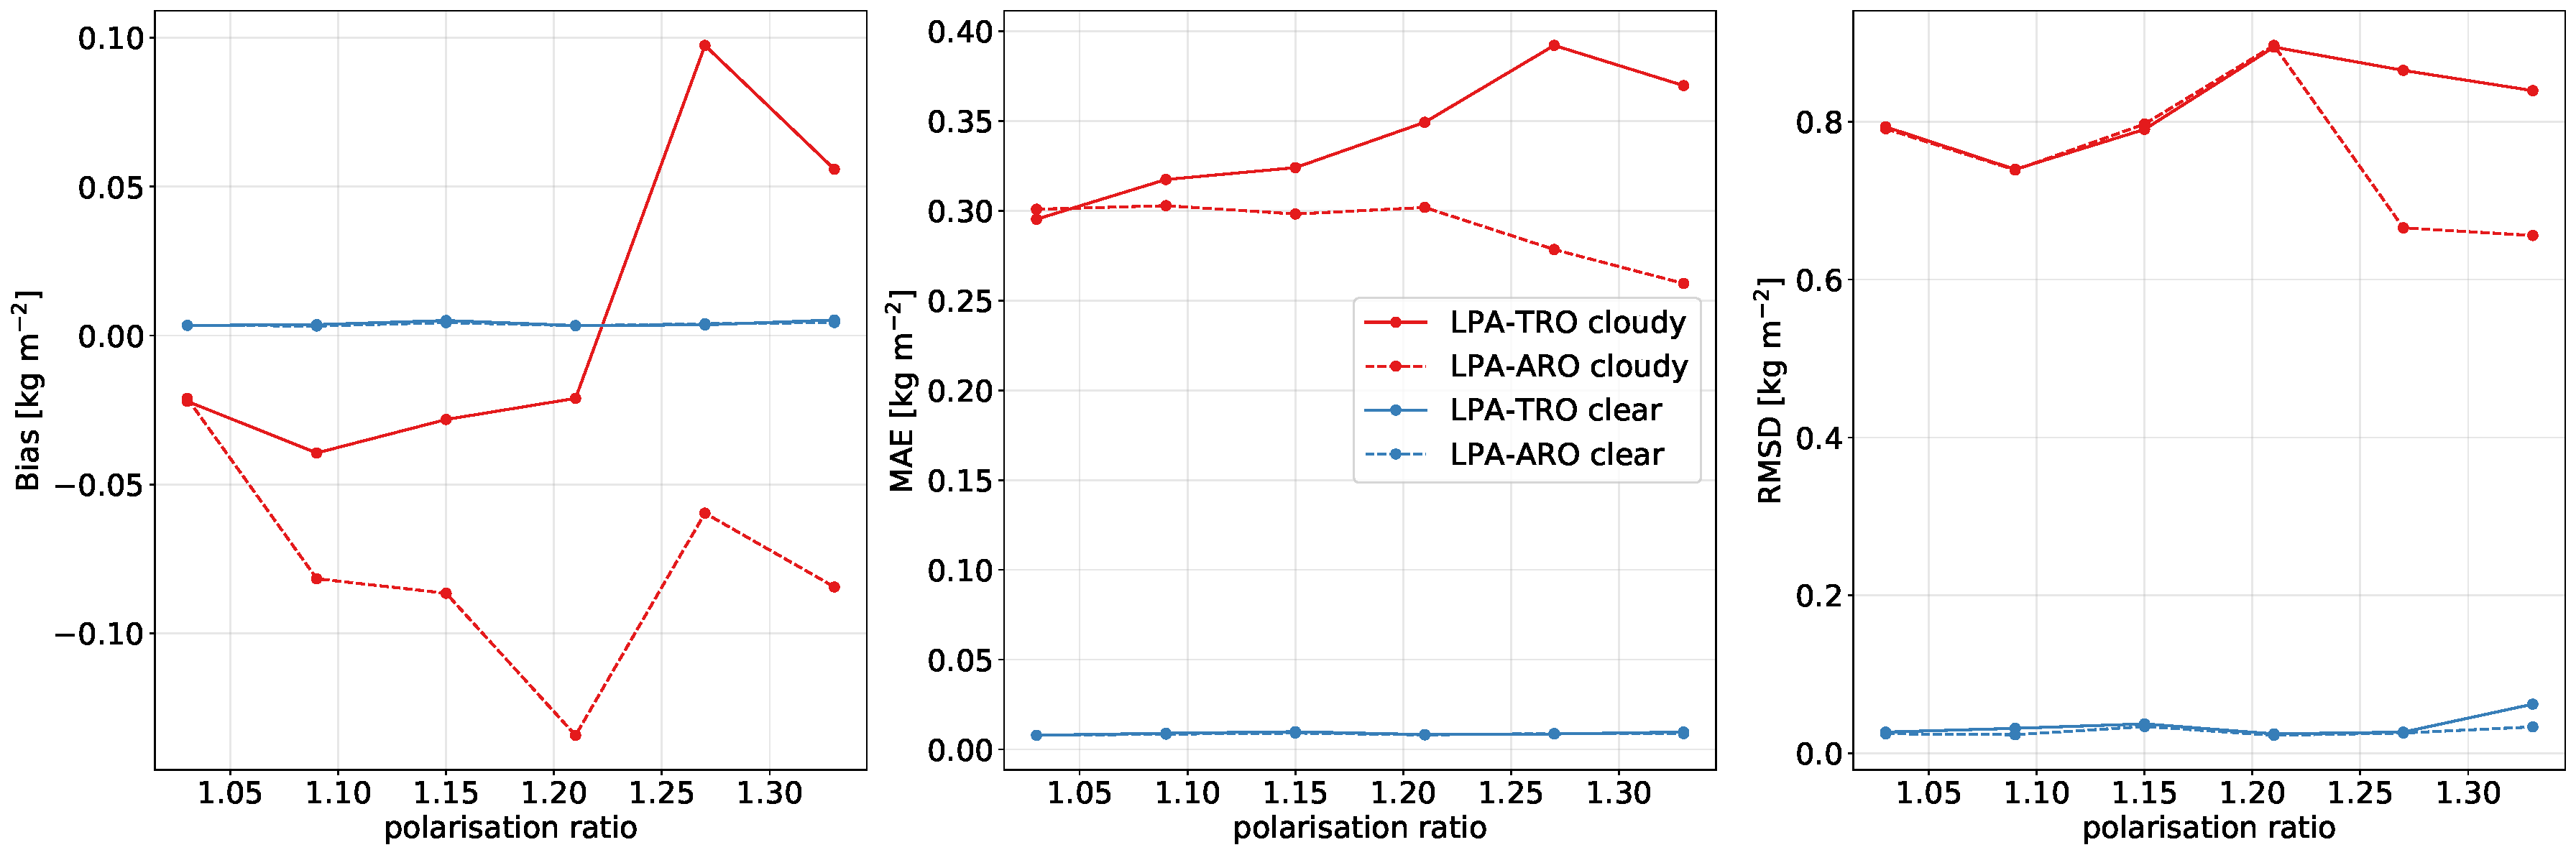
\includegraphics[width=12cm]{Figures/statistics_cloudyclear_LPA.pdf}
	\caption{}
	\label{fig:clear_cloudy}
\end{figure*}

\begin{figure}[t]
	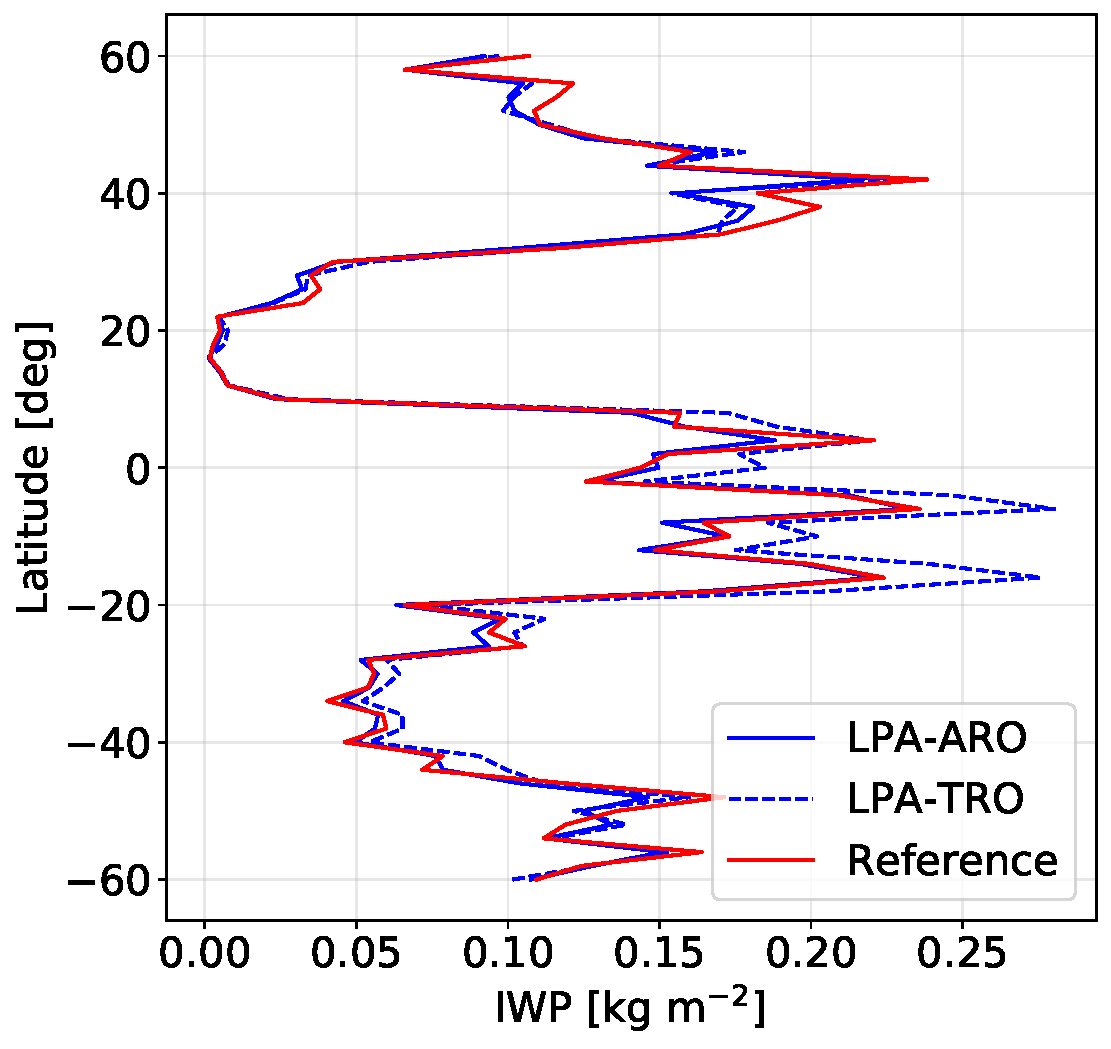
\includegraphics[width=8.3cm]{Figures/zonal_mean_all_jan_testdata.pdf}
	\caption{}
	\label{fig:zonal_mean_test}
\end{figure}

\begin{figure*}[t]
	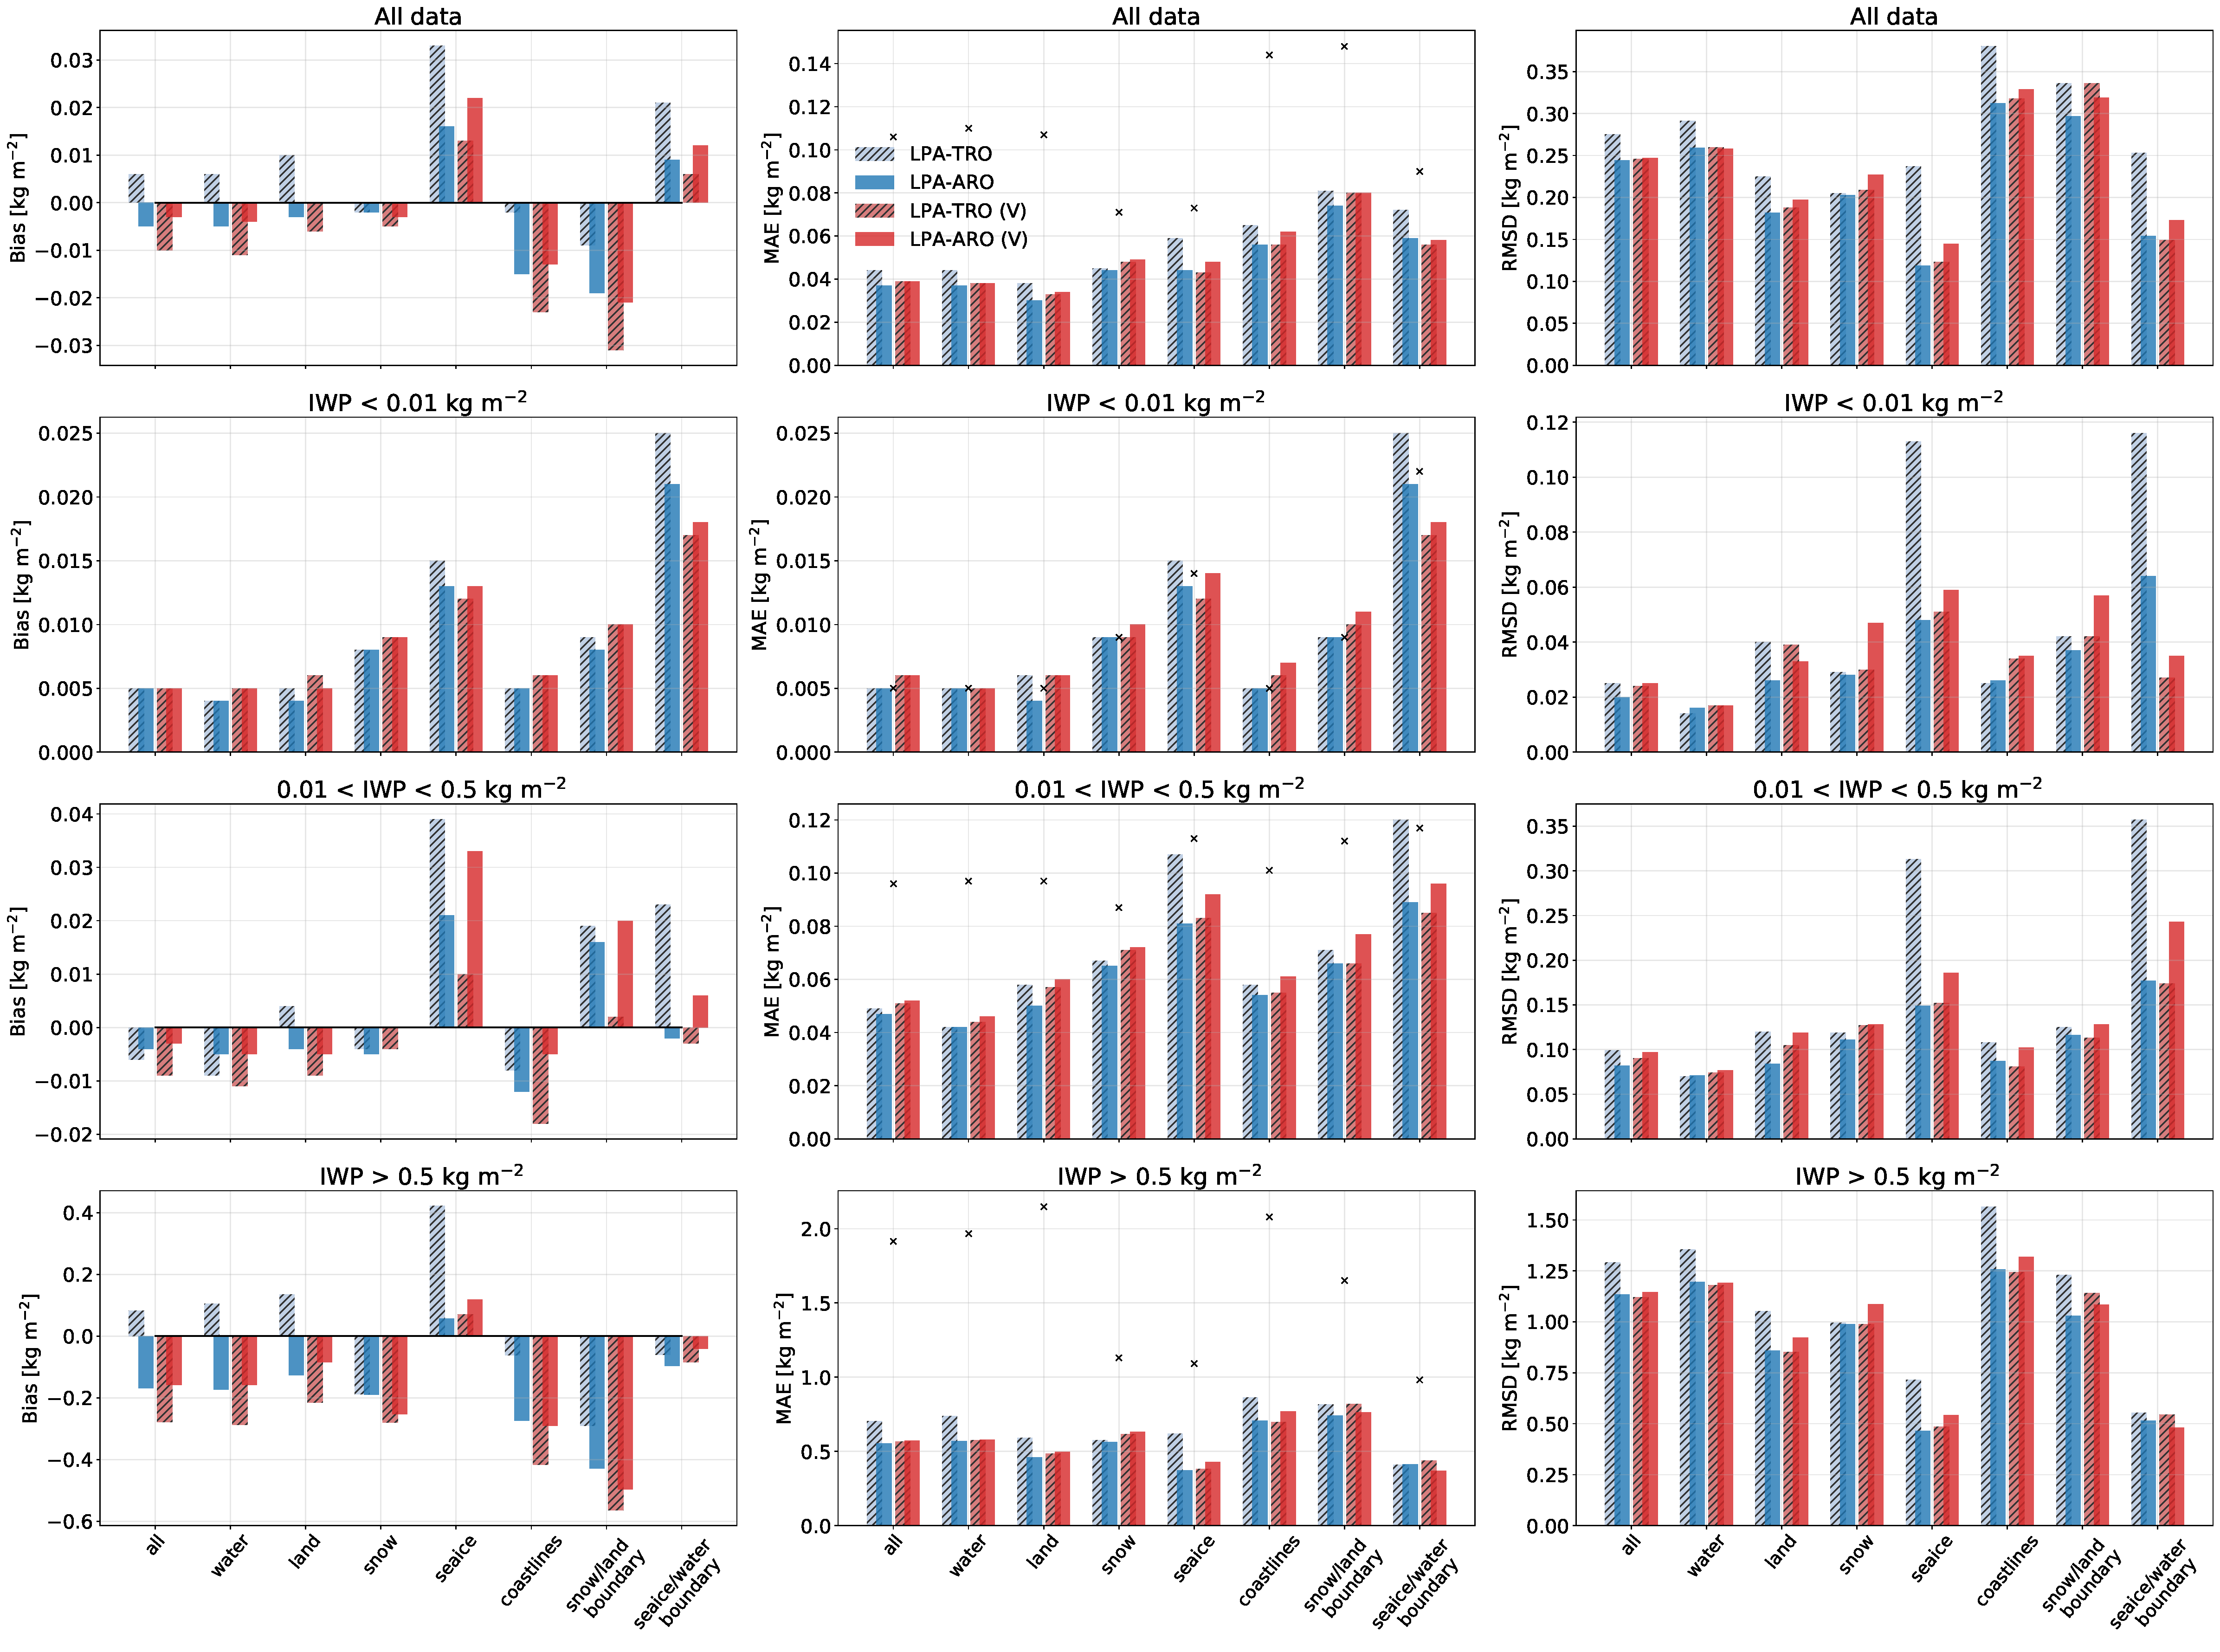
\includegraphics[width=12cm]{Figures/ARO_TRO_v_vh.pdf}
	\caption{}
	\label{fig:bias_ARO_TRO}
\end{figure*}

Figure~\ref{fig:clear_cloudy} shows the error statistics for retrievals based on ARO and TRO data based databases binned for different values of $\rho$. The retrieved data has been binned according to $\rho$ and divided into cloudy and clear-sky according to the reference IWP. All IWPs below 0.01\,\,kg m$^{-2}$ are classified as clear-sky, and vice-versa. For clear sky cases, $\rho$ has a negligible impact on the accuracy of the retrievals. The low IWPs are slightly overestimated as indicated by the low positive bias. On the other hand, for cloudy cases, a strong dependency of the accuracy on $\rho$ is observed. For $\rho = 1$ the both retrieval sets have similar accuracy. As $\rho$ increases up to 1.2, the bias in LPA-TRO is lower than LPA-ARO, but MAE shows slightly better accuracy for LPA-ARO. At the same time, RMSD remains unchanged between the two. However for $\rho > 1.20$, the differences between the two retrievals are most pronounced. The bias increases from -0.04 to 0.03 for $\rho = 1.35$, indicating an increase in the magnitude of IWP retrievals. This overestimation reduces the accuracy as indicated by the MAE and RMSD values. For $\rho = 1.35$ the RMSD increases by almost 25\%. This is not unexpected as this part of the distribution cannot be represented by TRO a priori distribution. But these statistics give an insight into the behaviour of IWP retrievals when scattering from cloud ice is neglected. Overall, neglecting oriented particles leads to an overestimation of the IWP. Figure~\ref{fig:zonal_mean_test}) gives an overview of the zonal averages from the both retrieval. The overestimation is largest over the tropics, where most ice clouds exist, but over higher latitudes, in both hemispheres, the differences between the two are small. This suggests that it is important to understand that if surface type has any impact on the retrieval accuracy. 

Figure~\ref{fig:bias_ARO_TRO} shows the bias and MAE values for these two retrievals for different surface types and different IWP ranges. Overall, the total bias between reference and retrievals increases from -0.005 to 0.006 when oriented particles are not included in the training.
Retrievals over land and water follow a similar trend. Over these two surface types, the performance of the two retrievals is quite similar for low IWP range, and the maximum differences between the two retrievals occur for high IWPs (> 1), where TRO based retrievals overestimate the IWPs. Both over land and water the bias increases by more than 100\%. Over snow, the overall retrievals seem bias free but high MAE values with respect to mean are seen. For seaice and seaice/water boundary, both retrievals are larger than the reference, though the average bias in LPA-TRO is twice as higher than LPA-ARO, and over seaice/water boundary the retrievals are thrice as higher. For both seaice, the overestimation of IWPs is observed over the entire dynamic range of IWP, but for the latter, most retrievals associated with clear-sky/low IWP are problematic. For coastlines the average bias increases from  -0.008\,\,kg m$^{-2}$ to -0.019\,\,kg m$^{-2}$ with inclusion of oriented particles, but the MAE reduces by almost 10\%.  

For IWPs < 0.1\,\,kg m$^{-2}$ the retrievals from both datasets are quite similar except for seaice and seaice boundary. For this range, the overall positive bias and MAE almost of the order of mean IWP show that most retrievals have an overestimation. This agrees well with the general behaviour of QRNN shown in sect.~\ref{sec:sec:basic_performance}.  

 

\paragraph{Including only V}
\label{sec:results_v}

In the previous section we showed the retrieval results from TRO and ARO based databases when dual-polarisation channels used. We now describe the retrieval differences when only V-polarised channel is used to train QRNN. 

Figure~\ref{fig:bias_ARO_TRO} (red bar plots) also shows the statistics for ARO and TRO based retrievals when only V-polarised channels is used. In contrast to results in the previous section, in this case, including impact of the oriented particles reduces the bias in IWP retrievals. A reduction in the bias is seen for all surface types except seaice and seaice boundary. For these two, the ARO based retrievals increases the positive bias, and the accuracy is also slightly reduced.

\subsection{Retrieval: GMI measurements}








\subsection{Discussion}



\conclusions  %% \conclusions[modified heading if necessary]
TEXT

%% The following commands are for the statements about the availability of data sets and/or software code corresponding to the manuscript.
%% It is strongly recommended to make use of these sections in case data sets and/or software code have been part of your research the article is based on.

\codeavailability{TEXT} %% use this section when having only software code available


\dataavailability{TEXT} %% use this section when having only data sets available


\codedataavailability{TEXT} %% use this section when having data sets and software code available


\sampleavailability{TEXT} %% use this section when having geoscientific samples available


\videosupplement{TEXT} %% use this section when having video supplements available


\appendix
\section{}    %% Appendix A

\subsection{}     %% Appendix A1, A2, etc.


\noappendix       %% use this to mark the end of the appendix section. Otherwise the figures might be numbered incorrectly (e.g. 10 instead of 1).

%% Regarding figures and tables in appendices, the following two options are possible depending on your general handling of figures and tables in the manuscript environment:

%% Option 1: If you sorted all figures and tables into the sections of the text, please also sort the appendix figures and appendix tables into the respective appendix sections.
%% They will be correctly named automatically.

%% Option 2: If you put all figures after the reference list, please insert appendix tables and figures after the normal tables and figures.
%% To rename them correctly to A1, A2, etc., please add the following commands in front of them:

\appendixfigures  %% needs to be added in front of appendix figures

\appendixtables   %% needs to be added in front of appendix tables

%% Please add \clearpage between each table and/or figure. Further guidelines on figures and tables can be found below.



\authorcontribution{TEXT} %% this section is mandatory

\competinginterests{TEXT} %% this section is mandatory even if you declare that no competing interests are present

\disclaimer{TEXT} %% optional section

\begin{acknowledgements}
TEXT
\end{acknowledgements}




%% REFERENCES

\bibliographystyle{copernicus}
\bibliography{references.bib}


%% Since the Copernicus LaTeX package includes the BibTeX style file copernicus.bst,
%% authors experienced with BibTeX only have to include the following two lines:
%%
%% \bibliographystyle{copernicus}
%% \bibliography{example.bib}
%%
%% URLs and DOIs can be entered in your BibTeX file as:
%%
%% URL = {http://www.xyz.org/~jones/idx_g.htm}
%% DOI = {10.5194/xyz}


%% LITERATURE CITATIONS
%%
%% command                        & example result
%% \citet{jones90}|               & Jones et al. (1990)
%% \citep{jones90}|               & (Jones et al., 1990)
%% \citep{jones90,jones93}|       & (Jones et al., 1990, 1993)
%% \citep[p.~32]{jones90}|        & (Jones et al., 1990, p.~32)
%% \citep[e.g.,][]{jones90}|      & (e.g., Jones et al., 1990)
%% \citep[e.g.,][p.~32]{jones90}| & (e.g., Jones et al., 1990, p.~32)
%% \citeauthor{jones90}|          & Jones et al.
%% \citeyear{jones90}|            & 1990



%% FIGURES

%% When figures and tables are placed at the end of the MS (article in one-column style), please add \clearpage
%% between bibliography and first table and/or figure as well as between each table and/or figure.

% The figure files should be labelled correctly with Arabic numerals (e.g. fig01.jpg, fig02.png).


%% ONE-COLUMN FIGURES

%%f
%\begin{figure}[t]
%\includegraphics[width=8.3cm]{FILE NAME}
%\caption{TEXT}
%\end{figure}
%
%%% TWO-COLUMN FIGURES
%
%%f
%\begin{figure*}[t]
%\includegraphics[width=12cm]{FILE NAME}
%\caption{TEXT}
%\end{figure*}
%
%
%%% TABLES
%%%
%%% The different columns must be seperated with a & command and should
%%% end with \\ to identify the column brake.
%
%%% ONE-COLUMN TABLE
%
%%t
%\begin{table}[t]
%\caption{TEXT}
%\begin{tabular}{column = lcr}
%\tophline
%
%\middlehline
%
%\bottomhline
%\end{tabular}
%\belowtable{} % Table Footnotes
%\end{table}
%
%%% TWO-COLUMN TABLE
%
%%t
%\begin{table*}[t]
%\caption{TEXT}
%\begin{tabular}{column = lcr}
%\tophline
%
%\middlehline
%
%\bottomhline
%\end{tabular}
%\belowtable{} % Table Footnotes
%\end{table*}
%
%%% LANDSCAPE TABLE
%
%%t
%\begin{sidewaystable*}[t]
%\caption{TEXT}
%\begin{tabular}{column = lcr}
%\tophline
%
%\middlehline
%
%\bottomhline
%\end{tabular}
%\belowtable{} % Table Footnotes
%\end{sidewaystable*}
%
%
%%% MATHEMATICAL EXPRESSIONS
%
%%% All papers typeset by Copernicus Publications follow the math typesetting regulations
%%% given by the IUPAC Green Book (IUPAC: Quantities, Units and Symbols in Physical Chemistry,
%%% 2nd Edn., Blackwell Science, available at: http://old.iupac.org/publications/books/gbook/green_book_2ed.pdf, 1993).
%%%
%%% Physical quantities/variables are typeset in italic font (t for time, T for Temperature)
%%% Indices which are not defined are typeset in italic font (x, y, z, a, b, c)
%%% Items/objects which are defined are typeset in roman font (Car A, Car B)
%%% Descriptions/specifications which are defined by itself are typeset in roman font (abs, rel, ref, tot, net, ice)
%%% Abbreviations from 2 letters are typeset in roman font (RH, LAI)
%%% Vectors are identified in bold italic font using \vec{x}
%%% Matrices are identified in bold roman font
%%% Multiplication signs are typeset using the LaTeX commands \times (for vector products, grids, and exponential notations) or \cdot
%%% The character * should not be applied as mutliplication sign
%
%
%%% EQUATIONS
%
%%% Single-row equation
%
%\begin{equation}
%
%\end{equation}
%
%%% Multiline equation
%
%\begin{align}
%& 3 + 5 = 8\\
%& 3 + 5 = 8\\
%& 3 + 5 = 8
%\end{align}
%
%
%%% MATRICES
%
%\begin{matrix}
%x & y & z\\
%x & y & z\\
%x & y & z\\
%\end{matrix}
%
%
%%% ALGORITHM
%
%\begin{algorithm}
%\caption{...}
%\label{a1}
%\begin{algorithmic}
%...
%\end{algorithmic}
%\end{algorithm}
%
%
%%% CHEMICAL FORMULAS AND REACTIONS
%
%%% For formulas embedded in the text, please use \chem{}
%
%%% The reaction environment creates labels including the letter R, i.e. (R1), (R2), etc.
%
%\begin{reaction}
%%% \rightarrow should be used for normal (one-way) chemical reactions
%%% \rightleftharpoons should be used for equilibria
%%% \leftrightarrow should be used for resonance structures
%\end{reaction}
%
%
%%% PHYSICAL UNITS
%%%
%%% Please use \unit{} and apply the exponential notation


\end{document}
